\documentclass[a4paper, 12pt, twoside]{report}

%% Language and font encodings
\usepackage[english]{babel}
\usepackage[utf8x]{inputenc}
\usepackage[T1]{fontenc}

%% Sets page size and margins
\usepackage[a4paper,top=3cm,bottom=2cm,left=2cm,right=2cm,bindingoffset = 2cm,marginparwidth=1.75cm]{geometry}

%% Useful packages
\usepackage{amsmath}
\usepackage{amssymb}
\usepackage{graphicx}
\usepackage{setspace}
\usepackage[colorinlistoftodos]{todonotes}
\usepackage[colorlinks=true, allcolors=blue]{hyperref}
\usepackage{color}
\usepackage{bm}
\usepackage{amsthm}
\usepackage{subfig}
\usepackage{mathtools}

\DeclarePairedDelimiter\floor{\lfloor}{\rfloor}

%Theorem environment
\newtheorem{theorem}{Theorem}[section]
\newtheorem{corollary}{Corollary}[theorem]
\newtheorem{lemma}[theorem]{Lemma}

\theoremstyle{definition}
\newtheorem{definition}{Definition}[section]

\title{An Advanced Numerical Algorithm for the Simulation of Weather Fronts}
\author{Chloe Raymont}
\newcommand{\comments}[1]{{\bfseries \color{red} Comment: #1 }}
\begin{document}
\begin{titlepage}

\newcommand{\HRule}{\rule{\linewidth}{0.5mm}} % Defines a new command for the horizontal lines, change thickness here

%----------------------------------------------------------------------------------------
%	LOGO SECTION
%----------------------------------------------------------------------------------------


\includegraphics[width=8cm]{title/logo.png}\\[1cm] % Include a department/university logo - this will require the graphicx package
 
%----------------------------------------------------------------------------------------

\center % Center everything on the page

%----------------------------------------------------------------------------------------
%	HEADING SECTIONS
%----------------------------------------------------------------------------------------

\textsc{\LARGE MSc Applied Mathematics Project\\ 2017/2018}\\[1.5cm] % Name of your university/college
\textsc{\Large Imperial College London}\\[0.5cm] % Major heading such as course name
\textsc{\large Department of Mathematics}\\[0.5cm] % Minor heading such as course title

%----------------------------------------------------------------------------------------
%	TITLE SECTION
%----------------------------------------------------------------------------------------
\makeatletter
\HRule \\[0.4cm]
{ \huge \bfseries \@title}\\[0.5cm] % Title of your document
\HRule \\[1.5cm]
 
%----------------------------------------------------------------------------------------
%	AUTHOR SECTION
%----------------------------------------------------------------------------------------

\begin{minipage}{0.4\textwidth}
\begin{flushleft} \large
\emph{Author:}\\
\@author % Your name
\end{flushleft}
\begin{flushleft} \large
	\emph{CID:}\\
	00733439 % CID
\end{flushleft}
\end{minipage}
~
\begin{minipage}{0.4\textwidth}
\begin{flushright} \large
\emph{Supervisor:} \\
Dr. Colin Cotter \\[1.2em] % Supervisor's Name
\end{flushright}
\end{minipage}\\[2cm]
\makeatother

% If you don't want a supervisor, uncomment the two lines below and remove the section above
%\Large \emph{Author:}\\
%John \textsc{Smith}\\[3cm] % Your name

%----------------------------------------------------------------------------------------
%	DATE SECTION
%----------------------------------------------------------------------------------------

{\large \today}\\[2cm] % Date, change the \today to a set date if you want to be precise

\vfill % Fill the rest of the page with whitespace

\end{titlepage}
\onehalfspacing
\begin{abstract}
This project studies the Eady Model for the formation of weather fronts in the atmosphere. Using the semi-geostrophic equations introduced by Hoskins \cite{Hoskins1975} by means of co-ordinate transform. A development to the transformation by Shutts and Cullen \cite{Shutts1987} leads to a form of the semi-geostrophic equations which can be reformulated as an optimal transport problem where the energy is the cost to be minimised \cite{Cullen2006a}. This is shown to be equivalent to an optimal transport problem minimising a quadratic cost. In this form we show that the Damped Newton Algorithm developed by Kitawaga et al. \cite{Kitagawa2016,Merigot2017a} for solving such problems can be applied. Numerical error and performance are subsequently analysed to validate results.
\end{abstract}

\renewcommand{\abstractname}{Acknowledgements}
\begin{abstract}

\end{abstract}
\renewcommand{\abstractname}{Declaration}
\begin{abstract}
	The work contained in this project is my own work unless otherwise stated.
	\begin{figure}[h]
		\centering
		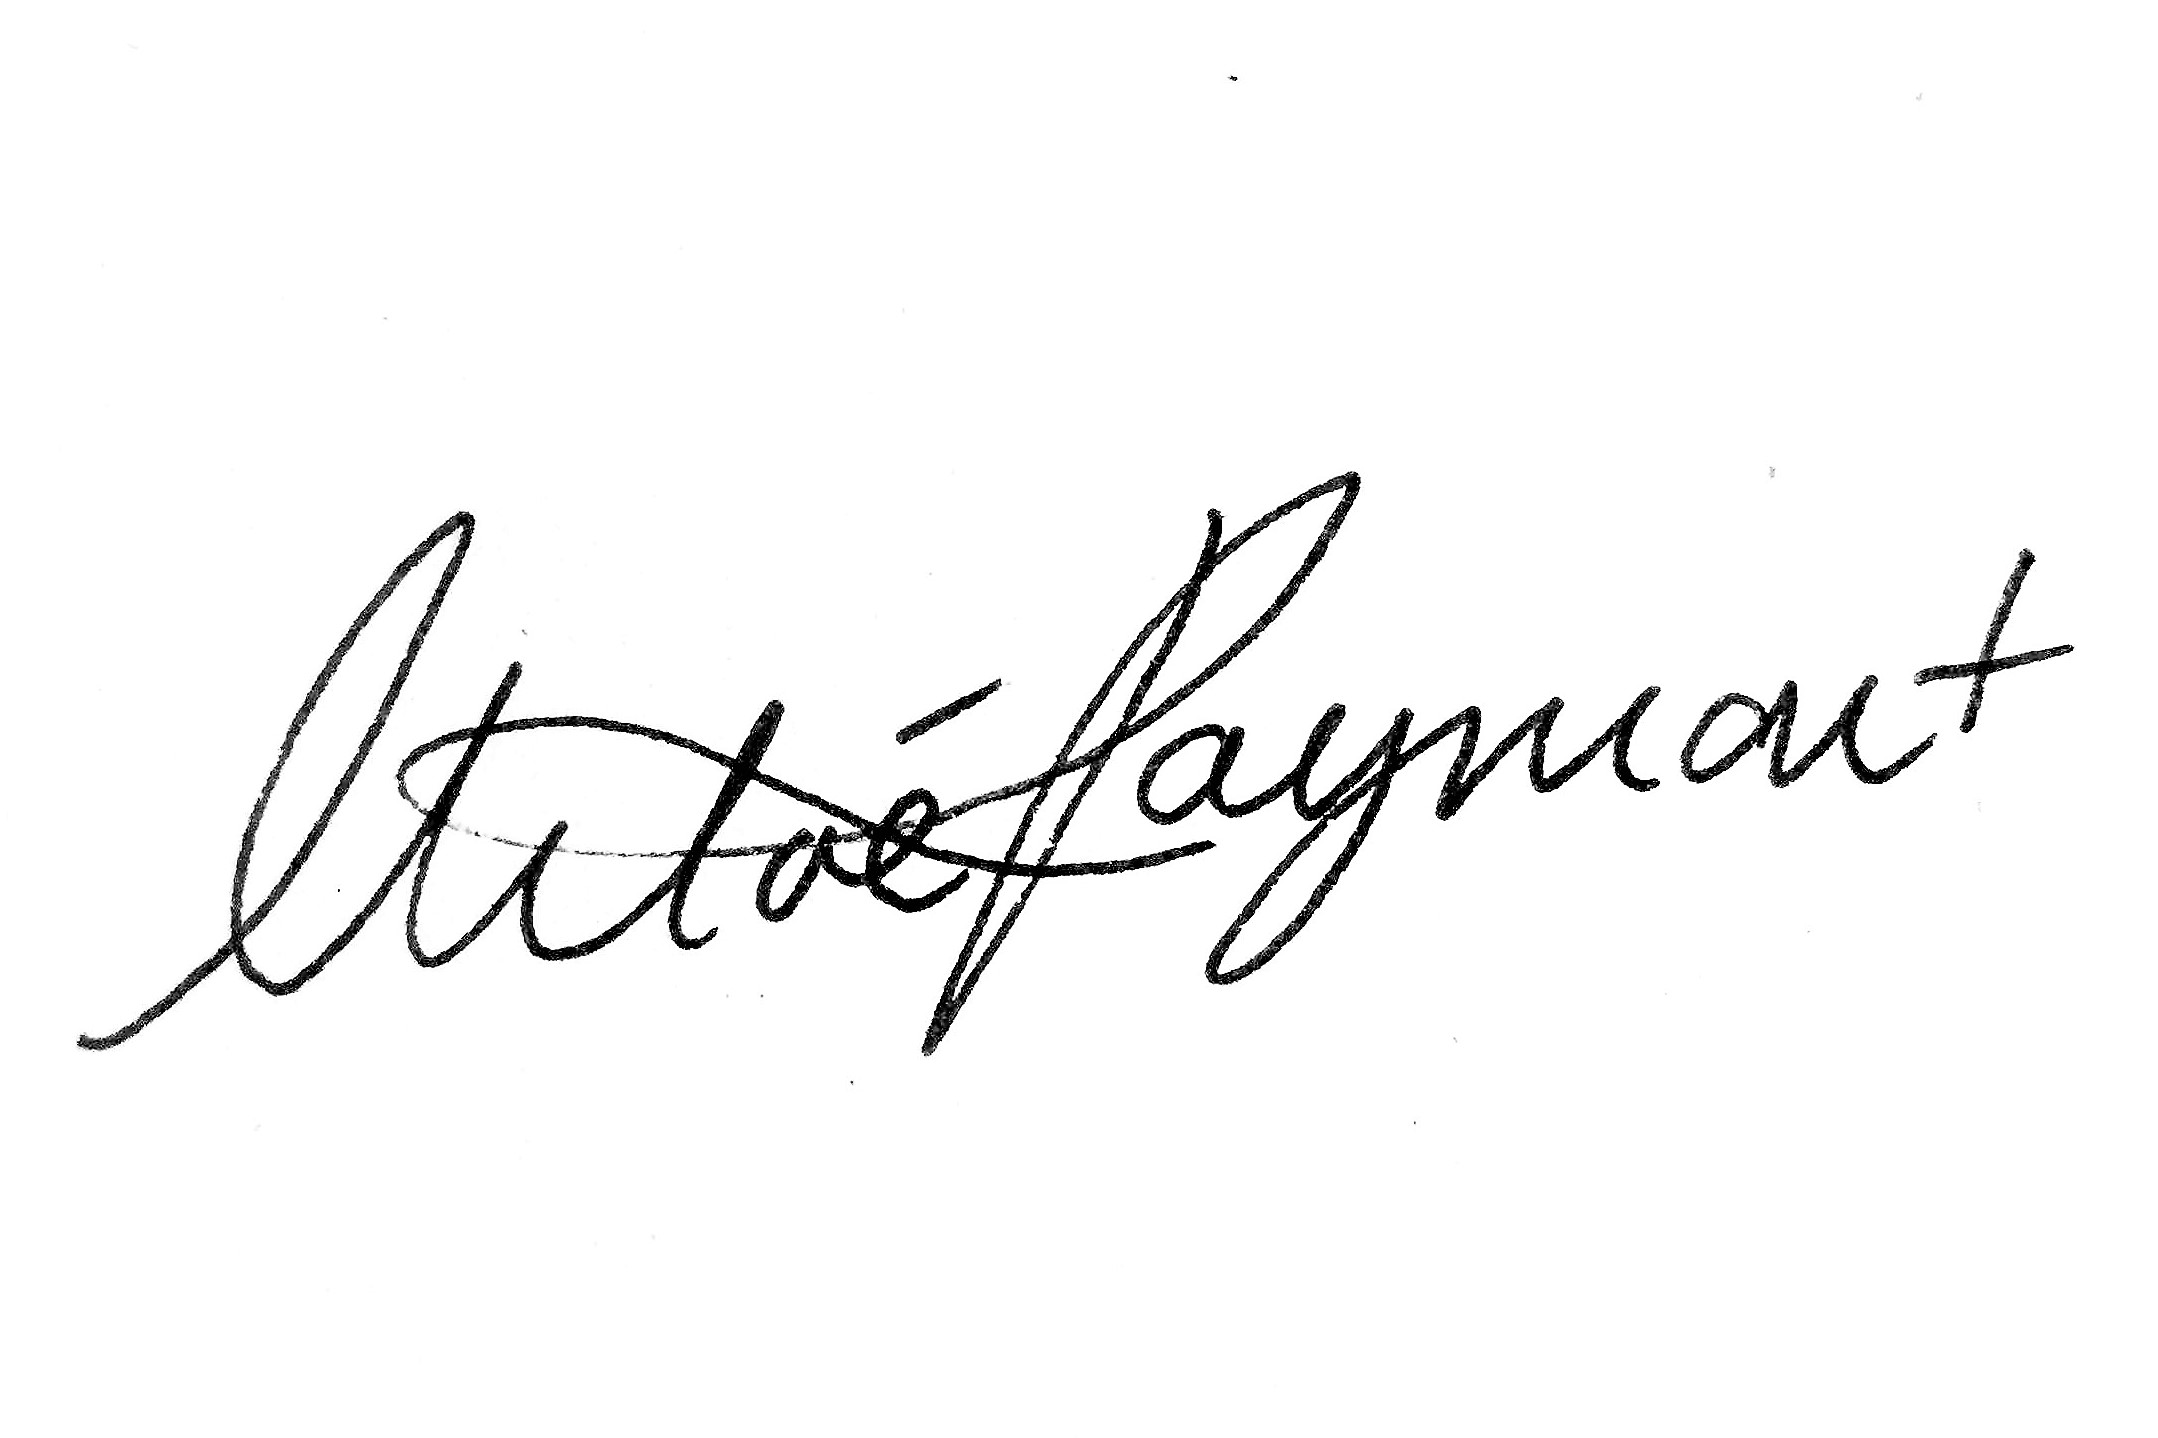
\includegraphics[width=0.7\linewidth]{ChloeRaymont_esignature}
	\end{figure}
	
\end{abstract}

\tableofcontents
\listoffigures
%\listoftables
\chapter*{Introduction}
\addcontentsline{toc}{chapter}{Introduction}
Numerical weather prediction (NWP) presents a rich area of research in geophysical fluid dynamics. With computer models continuing to provide larger range predictions \cite{Cullen2006a} questions arise as to the limit of predictability. Whilst the mathematical theory underlying NWP has been in place as early as the 1900s \cite{Golding2004}, predictions were limited by the capabilities of available technology. Of course, this is not the only limitation with chaos theory and the assimilation of observed data to be considered equally \cite{Weisheimer}. The increasing impact of extreme weather events on the world population means there is a vested interest in improving the predictability of NWP.
\\
\linebreak
This report is concerned developing a numerical modelling the formation of weather fronts, termed as frontogenesis{\tiny }. We study this process under the Semi-Geostrophic (SG) Vertical Slice Eady model (SG/EM), the governing equations for which we develop in Chapter \ref{governingequations}. As discussed by Mike Cullen in \cite{Cullen2006a} SG theory provides a highly predictable, general system for the study of large-scale atmospheric flow. With no formal mathematical definition we follow \cite{Hoskins1982}, where fronts are considered as regions that have length scales comparable to the height of the domain considered, whilst exhibiting large gradients in other variables in the cross direction. Frontogenesis has been studied extensively \cite{Yamazaki2017, Cullen2008, Rotunno1994,Nakamura1988,Nakamura1994}, naturally, as it features heavily in large-scale atmosphere flow (of the order 1000km) \cite{Cullen2006a}.
\\
\linebreak
Work by B. Hoskins expressed the SG equations in \textquoteleft geostrophic co-ordinates\textquoteright \ \cite{Hoskins1972}. This was subsequently developed by Shutts and Cullen \cite{Shutts1987}. In this framework the SG equations exhibit interesting geometrical properties. Namely it was shown that solutions can be sought as those of an equivalent Monge-Amp\`{e}re/Optimal Transport problem \cite{Cullen2006a}. This reformulation is discussed in chapter \ref{Chapter3}.
\\
\linebreak
Our focus now shifts to the numerical solution of SG/EM through optimal transport methods. In this report following the suggestion of Dr Cotter, a solution using the Damped Newton Algorithm (DA) recently developed by M\`{e}rigot et al. \cite{Merigot2017, Merigot2017a, Kitagawa2016} is explored. This was shown to be particularly efficient in solving optimal transport problems of the Monge-Amp\`{e}re type. In Chapter \ref{OptimalTransport} we highlight the suitability of DA in solving the SG/EM equations for frontogenesis, and subsequently discuss how this is achieved in Chapter \ref{algorithm}.
\\
\linebreak
Finally, in Chapter \ref{results} we aim to validate the suitability of this numerical algorithm in solving SG/EM. This will be done through suitable analysis of the error as well as comparison to results produced by other numerical models under similar conditions \cite{Nakamura1994,Cullen1993}.


\chapter{The Governing Equations \label{governingequations}}
The semi-geostrophic equations first introduced by \cite{Eliassen1962}
form the basis of our model for frontogenesis. Widely noted to provide results more frequently observed than the classical quasi-geostrophic equations in their description of the formation of weather fronts 
\cite{Cullen2006a, Hoskins1975}. 
In this chapter a summary of key steps that lead to the Eady model for frontogensis that was developed by Hoskins and Bretherton , 1972, \cite{Hoskins1972} is given. Based on the model for baroclinic instability proposed by Eady, 1949, incorporating a linear stratification in density and a constant vertical shear in the horizontal velocity component. A co-ordinate transform to geostrophic co-ordinates by  \cite{Hoskins1975} 
facilitates the numerical implementation of these equations and subsequent interpretation of results. For the following the main points are summarised from Cullen 2006 \cite{Cullen2006a} in formulating the model to be implemented numerically.
\section{The Semi-Geostrophic Equations \label{SGeqns}} 
\subsection{The 3D Incompressible Boussinesq Equations}
\begin{figure}[h]
	\centering
	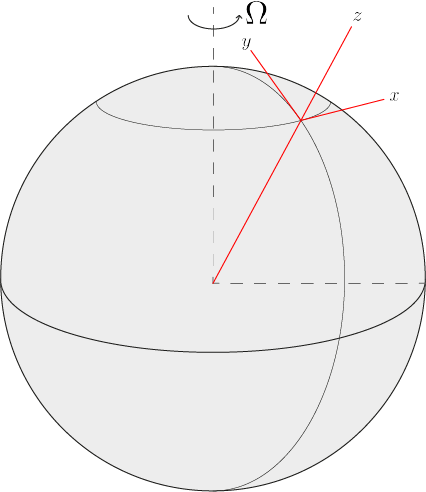
\includegraphics[width=5cm]{background/local_cartesian}
	\caption{Local cartesian co-ordinates $\left(x,y,z\right)$ on Earth}
	\label{fig:localcartesian}
\end{figure}
We begin with the $3$D incompressible Boussinesq equations \ref{3DBous} to describe atmospheric flow. Adopting cartesian co-ordinates $\left(x,y,z\right)$ representing the zonal, meridional and radial directions on the Earth respectively, as shown in \ref{fig:localcartesian}. The corresponding velocity components are $\bm{u}=\left(u,v,w\right)$, with $\rho_0$ representing the constant density and $p$ denoting the pressure.
\begin{equation}
	\begin{aligned}
		\frac{\mathrm{D}u}{\mathrm{D}t}	- fv  &= -\frac{1}{\rho_0}\frac{\partial p}{\partial x}\\
		\frac{\mathrm{D}v}{\mathrm{D}t}	+ fu  &= -\frac{1}{\rho_0}\frac{\partial p}{\partial y}\\
		\frac{\mathrm{D}w}{\mathrm{D}t} &= -\frac{1}{\rho_0}\frac{\partial p}{\partial z} + b\\
		\frac{\mathrm{D} b}{\mathrm{D}t} &= 0\\
		\nabla \cdot \bm{u} &= 0
	\end{aligned}
\label{3DBous}
\end{equation}
Under the Boussinesq assumption that density fluctuations are small, the thermodynamic equation is written as equation (4) in the system above. The buoyancy is characterised by Potential Temperature, $\theta$ as $b = \frac{g\theta}{\theta_0}$. By also introducing the geopotential $\phi = \frac{p}{\rho_0}$, equations \ref{3DBous} are rewritten as
\begin{equation}
	\begin{aligned}
		\frac{\mathrm{D}u}{\mathrm{D}t}	- fv  &= -\frac{\partial \phi}{\partial x}\\
		\frac{\mathrm{D}v}{\mathrm{D}t}	+ fu  &= -\frac{\partial \phi}{\partial y}\\
		\frac{\mathrm{D}w}{\mathrm{D}t} &= -\frac{\partial \phi}{\partial z} + \frac{g\theta}{\theta_0}\\
		\frac{\mathrm{D} \theta}{\mathrm{D}t} &= 0\\
		\nabla \cdot \bm{u} &= 0
	\end{aligned}
\label{3DBousPT}
\end{equation}
where $\theta_0$ and $g$ denote initial potential temperature and acceleration due to gravity respectively. \\
$\frac{\mathrm{D}}{\mathrm{D}t} \equiv \frac{\partial}{\partial t} + u\frac{\partial}{\partial x} + v\frac{\partial}{\partial y} + w\frac{\partial}{\partial z},\qquad$ 
$\nabla \equiv \left(\frac{\partial}{\partial x}, \frac{\partial}{\partial y},\frac{\partial}{\partial z}\right)$ \\
\linebreak
Additionally if the hydrostatic approximation, that vertical acceleration is small compared to gravity, so that, $\frac{\mathrm{D}w}{\mathrm{D}t} = 0$. Then, 
\begin{equation}
	\begin{aligned}
	\frac{\mathrm{D}u}{\mathrm{D}t}	- fv  &= -\frac{\partial \phi}{\partial x}\\
	\frac{\mathrm{D}v}{\mathrm{D}t}	+ fu  &= -\frac{\partial \phi}{\partial y}\\
	-\frac{\partial \phi}{\partial z} + \frac{g\theta}{\theta_0} &= 0\\
	\frac{\mathrm{D} \theta}{\mathrm{D}t} &= 0\\
	\nabla \cdot \bm{u} &= 0
	\end{aligned}
	\label{3DBousPThydro}
\end{equation}
\subsection{The Vertical Slice Model}
To facilitate the study of frontogenesis a vertical slice model is introduced. In this report the vertical slice is defined as the $\left(x-z\right)$ plane. The domain considered is defined as, $\Gamma := [-L,L] \times [0,H]$. Perturbations to the leading-order fields are considered as functions of $x,z$ and $t$ only, whereas the leading order terms in $\theta$ and $\phi$ are functions of $\left(y,z\right)$. Retaining the potential temperature gradient normal to the slice is crucial to the subsequent evolution of the front. Following the ideas of Yamazaki, 2017 \cite{Yamazaki2017} we introduce,
\begin{equation}
	\begin{aligned}
		\theta = \bar{\theta}(y,z) + \theta'(x,z,t)\\ 
		\phi = \bar{\phi}(y,z) + \varphi(x,z,t)\\
		\bm{u} = \bar{\bm{u}}(y,z) + \bm{u}'(x,z,t)
	\end{aligned}
\label{perturbations for vertical slice}
\end{equation}
With the background field for $\theta$ chosen as,
\begin{equation}
	\begin{aligned}
		\bar{\theta} &= -Cy
	\end{aligned}
\label{bgTP}
\end{equation}
Where $\frac{\partial \theta}{\partial y} = -C$ is a constant, normal to the slice potential temperature gradient.\\
\linebreak
The background field for $\phi$ is chosen so that both background fields for $\theta $ and $\phi $ satisfy the third equation of \ref{3DBousPThydro},
\begin{equation*}
	-\frac{\partial \bar{\phi}}{\partial z} + \frac{g\bar{\theta}}{\theta_0} = 0
\end{equation*}
with the boundary condition $\phi = 0$ at $z = H/2$. This gives,
\begin{equation}
	\bar{\phi} = -\frac{Cgy}{\theta_0}\left(z - H/2\right)
\label{bgphi}
\end{equation}
\comments{not here:}
The Brunt-V\"{a}is\"{a}l\"{a} frequency $N^2 = \frac{g}{\theta_0}\frac{\partial \theta}{\partial z}$ characterises the stratification of density in the slice.\\
\linebreak
To reach the vertical slice model we substitute the forms \ref{perturbations for vertical slice} with expressions for the background fields \ref{bgTP} and \ref{bgphi} into equations \ref{3DBousPThydro}. 
\begin{equation}
	\begin{aligned}
		\frac{\mathrm{D}u}{\mathrm{D}t}	- fv  &= -\frac{\partial}{\partial x}\left(\bar{\phi} + \varphi\right)
		\\
		\frac{\mathrm{D}v}{\mathrm{D}t}	+ fu  &= -\frac{\partial}{\partial y}\left(\bar{\phi} + \varphi\right)
		\\
		0 &=\frac{\partial}{\partial z}\left(\bar{\phi} + \varphi\right) - \frac{g}{\theta_0}\left(\bar{\theta} + \theta'\right)
		\\
		0 & =\frac{\partial }{\partial t}\left(\bar{\theta} + \theta'\right) +u\frac{\partial }{\partial x}\left(\bar{\theta} + \theta'\right) + v\frac{\partial }{\partial y}\left(\bar{\theta} + \theta'\right) + w\frac{\partial }{\partial z}\left(\bar{\theta} + \theta'\right)
		\\
		0 &= \frac{\partial u}{\partial x} + \frac{\partial v}{\partial y} + \frac{\partial w}{\partial z}
	\end{aligned}
\end{equation}
By neglecting $\partial/\partial y$ terms except in background variables, after rearrangement the vertical slice equations are obtained as,
\begin{equation}
	\begin{aligned}
		\frac{\partial u}{\partial t} + u\frac{\partial u}{\partial x} + w\frac{\partial u}{\partial z}	- fv  &= -\frac{\partial \varphi}{\partial x}
		\\
		\frac{\partial v}{\partial t} + u\frac{\partial v}{\partial x} + w\frac{\partial v}{\partial z}	+ fu  &= -\frac{\partial \varphi}{\partial y} + \frac{Cg}{\theta_0}\left(z - H/2\right)
		\\
		0 &=\frac{\partial \varphi}{\partial z} - \frac{g\theta'}{\theta_0}
		\\
		0 & =\frac{\partial \theta'}{\partial t} + u\frac{\partial \theta'}{\partial x} - Cv + w\frac{\partial \theta'}{\partial z}
		\\
		0 &= \frac{\partial u}{\partial x} + \frac{\partial w}{\partial z}
	\end{aligned} 
\label{VerticalSlice}
\end{equation}
By redefining the material derivative operator as $\frac{\mathrm{D} }{\mathrm{D} t} \equiv \frac{\partial  }{\partial t} + u\frac{\partial  }{\partial x} + w\frac{\partial  }{\partial z} $, and gradient operator $\nabla = \left(\frac{\partial }{\partial x}, \frac{\partial }{\partial z}\right)$
\begin{equation}
	\begin{aligned}
	\frac{\mathrm{D}u}{\mathrm{D}t}	- fv  &= -\frac{\partial \varphi}{\partial x}
	\\
	\frac{\mathrm{D}v}{\mathrm{D}t}	+ fu - \frac{Cg}{\theta_0}\left(z - H/2\right) &= -\frac{\partial \varphi}{\partial y} 
	\\
	\frac{\partial \varphi}{\partial z} - \frac{g\theta'}{\theta_0} &= 0
	\\
	\frac{\mathrm{D}\theta'}{\mathrm{D} t}  - Cv &= 0
	\\
	\nabla \cdot \bm{u} &= 0
	\end{aligned} 
\label{VerticalSlice2}
\end{equation}
\subsection{The Geostrophic Momentum Approximation \label{Geostrophic}}
To reach the final semi-geostrophic Eady model for frontogenesis the Geostrophic Momentum approximation is made. Developed by Hoskins, 1975 \cite{Hoskins1975}, where further detail can be found, the following section gives a brief summary of the key arguments.\\
\linebreak
Going back to equations \ref{3DBousPT}. We consider an expansion in the Rossby number $\epsilon = U/fL$ where $U$ and $L$ are horizontal velocity and length scaled respectively. Expanding the momentum equations in \ref{VerticalSlice2} in leading-order (geostrophic) and first order (ageostrophic) terms in $\epsilon$, so that,
\begin{equation*}
	\bm{u} = \bm{u_g} + \epsilon \bm{u_a} \qquad \varphi = \varphi_g +\epsilon \varphi_a
\end{equation*}
Acceleration terms are found to be $O(\epsilon)$ so that at the leading order the geostrophic balance is found to be,
\begin{equation}
	fv_g  = -\frac{\partial \varphi_g}{\partial x} \qquad
	-fu_g  = -\frac{\partial \varphi_g}{\partial y}
\end{equation}
Subsequent analysis as detailed in Hoskins 1975, \cite{Hoskins1975} finds the prognostic equations for ageostrophic variables to be such that the momentum $\frac{\mathrm{D}u}{\mathrm{D}t}, \frac{\mathrm{D}v}{\mathrm{D}t}$ are replaced with their geostrophic counterparts $\frac{\mathrm{D}u_g}{\mathrm{D}t}, \frac{\mathrm{D}v_g}{\mathrm{D}t}$. Noting that in the vertical slice model $u_g = 0$ we find equations \ref{VerticalSlice} with the geostrophic momentum approximation as
\begin{equation}
	\begin{aligned}
		-fv_g + \frac{\partial \varphi}{\partial x} = 0,\\
		\frac{Dv_g}{Dt} + fu -\frac{Cg}{\theta _0}\left(z-H/2\right) = 0,\\
		\frac{D\theta'}{Dt} - Cv_g = 0,\\
		\frac{\partial \varphi}{\partial z} - g\frac{\theta'}{\theta_0} = 0,\\
		\nabla \cdot \bm{u} = 0.
	\end{aligned}
\label{EadyModel}
\end{equation}
\comments{First equation is different - $-fv_g$ isn't $O(\epsilon)$??}
Where, for convenience the subscript denoting ageostrophic variables has been dropped. \\
\linebreak
The corresponding energy integral given by \cite{Cullen2006a} is,
\begin{equation}
	E = \iint_{\Gamma} \frac{1}{2}v_g^2 - \frac{g\theta'}{\theta_0}\left(z - H/2\right)\textrm{d}x\textrm{d}z
\end{equation}
Equations \ref{EadyModel} form the basis of the subsequent investigation of frontogenesis in this report. They are to be solved over the domain $\Gamma = [-L,L] \times [0,H]$, with the periodic boundary conditions in $x$ and the rigid-lid boundary condition $w = 0$ on $z = 0,H$. \\
\linebreak
The front formation seen later in the report is a consequence of a baroclinic instability introduced by Cullen 2006 \cite{Cullen2006a} in the form of a perturbation to $\theta'$, 
\begin{equation}
	\theta' = \frac{N^2\theta_0 z}{g} + B\sin\left(\pi\left(x/L + z/H\right)\right)
\label{thetap}
\end{equation}
\comments{does this need including?}
\begin{itemize}
	\item \textbf{Key Scalings}
	It is worth noting that Eady's original model for baroclinic instability was developed under a quasi-geostrophic model, where $\epsilon = Fr \ll 1$ in contrast semi-geostrophic theory the assumes, $\epsilon \ll 1$ with $\epsilon < Fr$.
\end{itemize}
\chapter{The Frontogenesis Model as an Optimal Transport Problem \label{Chapter3}}
The semi-geostrophic equations have previously been rigorously analysed \cite{Hoskins1975,Bannon1988,Cullen1993} and models subsequently developed to include momentum diffusion \cite{Blumen1990, Nakamura1994}. The existence of smooth solutions for the Eady Model for frontogenesis \ref{EadyModel} is shown in \cite{Brenier2009}. Perhaps one of the most exciting developments in the study of frontogenesis was the reformulation of the semi-geostrophic equations into a Monge-Amp\`{e}re equation for mass transportation \cite{Benamou1998} \comments{CHECK!}. It is shown in \cite{Cullen2006a} that a through a transformation to geostrophic co-ordinates as described in section \ref{Geostrophic} the energy integral can be viewed as the 'cost' in a moss transportation problem. This reformulation has allowed a deeper insight into the behaviour of the equations through numerical solutions developed from methods in computational geometry. In this chapter the arguments given in \cite{Cullen2006a} are summarised to highlight the application of optimal transport theory to the Eady Model for frontogenesis \ref{EadyModel}.
\comments{smooth solutions only in geostrophic co-ordinates}
\section{Transformation to Geostrophic Co-ordinates \label{transformation}}
To facilitate the implementation of the numerical scheme we will subsequently use to solve equations \ref{EadyModel} we transform to geostrophic co-ordinate system first introduced by Hoskins \cite{Hoskins1975} in the horizontal directions $(x,y)$. The geostrophic co-ordinates describe the position of particles had they evolved under their geostrophic velocity. This transformation was later developed by Cullen \cite{Cullen2006a} to include a transformation in terms of $\theta '$ in the vertical direction. The geostrophic transformation $\Phi: (x,z) \rightarrow (X,Z)$
\begin{equation}
X = x + \frac{v_g}{f}, \qquad Z = \frac{g\theta'}{f^2\theta_0}
\end{equation}
By defining
\begin{equation}
P = \frac{1}{2}x^2 + \frac{1}{f^2}\varphi
\label{P}
\end{equation}
It is clear that,
\begin{equation*}
\begin{aligned}
\nabla P &= \left(x + \frac{1}{f^2}\frac{\partial \varphi}{\partial x}, \frac{1}{f^2} \frac{\partial \theta'}{\partial z}\right)
&= \left(x + \frac{v_g}{f}, \frac{g\theta'}{f^2\theta_0}\right)
\end{aligned}
\end{equation*}
So that upon substitution from the first and fourth equations in \ref{EadyModel} we find,
\begin{equation}
\nabla P = (X,Z)
\label{gradP}
\end{equation}
By noting that,
\begin{equation*}
\frac{\mathrm{D}X}{\mathrm{D}t} = \frac{\mathrm{D}x}{\mathrm{D}t} + \frac{1}{f}\frac{\mathrm{D}v_g}{\mathrm{D}t} = u + \frac{1}{f}\frac{\mathrm{D}v_g}{\mathrm{D}t}, \qquad \frac{\mathrm{D}Z}{\mathrm{D}t} = \frac{g}{f^2\theta_0} \frac{\mathrm{D}\theta '}{\mathrm{D}t}
\end{equation*}
the momentum equations from \ref{EadyModel} are transformed into geostrophic co-ordinates as
\begin{equation}
\frac{\mathrm{D}X}{\mathrm{D}t} -\frac{Cg}{f\theta _0}\left(z-H/2\right) = 0,\qquad
\frac{\mathrm{D}Z}{\mathrm{D}t} - \frac{Cg}{f\theta_0}\left(X - x\right) = 0,
\label{Gmom}
\end{equation}
It is also shown in \cite{Cullen2006a} that the continuity equation holds in geostrophic co-ordinates. with $\bm{U} = \frac{Cg}{f\theta _0}\left(z-H/2, X-x\right) $
Putting together equations \ref{P}, \ref{gradP}, \ref{Gmom} the Eady Model in geostrophic co-ordinates is 
\begin{equation}
\begin{aligned}
\frac{\mathrm{D}X}{\mathrm{D}t} -\frac{Cg}{f\theta _0}\left(z-H/2\right) = 0 \\
\frac{\mathrm{D}Z}{\mathrm{D}t} - \frac{Cg}{f\theta_0}\left(X - x\right) = 0,\\
P = \frac{1}{2}x^2 + \frac{1}{f^2}\varphi,\\
\nabla P = (X,Z)\\
\nabla \cdot \bm{U} = 0
\end{aligned}
\label{EadyGC}
\end{equation}
The corresponding energy integral given by transforming the Energy \ref{energy} with \ref{transformation} is,
\begin{equation}
E = f^2 \iint \frac{1}{2}\left(X-x\right)^2 - Z\left(z - H/2\right)\textrm{d}x\textrm{d}z
\label{energy}
\end{equation}
\section{Energy Minimisation as an Optimal Transportation Problem}
It is shown in \cite{Cullen2006a} and references therein that the hydrostatic and geostrophic balances in the Semi-geostrophic equations characterise the solution as an Energy minimisation problem. In geostrophic co-ordinates, Theorem 3.3 from \cite{Cullen2006a} the condition to minimise the energy \ref{energy} is that the function $P$ is convex. In this section we show that this can be reformulated to take the form of an optimal transport problem with quadratic cost. This amounts to the solution of \ref{EadyGC} as finding $\left(X, Z\right)$ which minimise the energy and subsequently finding their time evolution using \ref{EadyGC}.
\subsection{Finding an Inverse Transformation}
Consider an initial set of points in geostrophic space $(X,Z)$. To find the trajectory of points in geostrophic space and consequently to solve \ref{EadyGC} requires the corresponding values $\left(x,z\right)$. This requires the existence of a unique inverse to the transform \ref{transformation}. Following \cite{Cullen2006a}, the function $R(X,Z)$ is defined as,
\begin{equation*}
	R(X,Z) = x(X,Z)X+z(X,Z)Z - P(x,y,z)
\end{equation*}
To rewrite the energy integral \ref{energy} in geostrophic co-ordinates requires the jacobian of the inverse transformation $\Phi ^{-1}: (X,Z) \rightarrow (x,z)$, 
\begin{equation}
	\sigma(X,Z) = \frac{\partial x}{\partial X}\frac{\partial z}{\partial Z} - \frac{\partial z}{\partial X}\frac{\partial x}{\partial Z}
\label{sigma defn}
\end{equation}
Noting that,
\begin{equation*}
	\frac{\partial R}{\partial X} = x + X\frac{\partial x}{\partial X} + Z\frac{\partial z}{\partial X} -\frac{\partial P}{\partial x}\frac{\partial x}{\partial X} - \frac{\partial P}{\partial x}\frac{\partial z}{\partial X}
\end{equation*}
Similarly,
\begin{equation*}
\frac{\partial R}{\partial Z} = X\frac{\partial x}{\partial Z} + z + Z\frac{\partial z}{\partial Z} -\frac{\partial P}{\partial Z}\frac{\partial x}{\partial Z} - \frac{\partial P}{\partial Z}\frac{\partial z}{\partial Z}
\end{equation*}
Using $\nabla P = (X,Z)$, we find,
\begin{equation}
	\nabla_{(X,Z)} R = \left(\frac{\partial R}{\partial X},\frac{\partial R}{\partial Z}\right) = (x,z)
\end{equation}
This is convenient as it allows us to rewrite \ref{sigma defn} as,
\begin{equation}
\sigma(X,Z) = \frac{\partial^2 R}{\partial X^2}\frac{\partial^2 R}{\partial Z^2} -\frac{\partial^2 R}{\partial XZ}\frac{\partial^2 R}{\partial ZX} = \textrm{det}(Hess \ R)
\label{Monge Ampere}
\end{equation}
As stated in \cite{Cullen2006a} this is a form of the classical \textbf{Monge Amp\`{e}re equation} for a given $\sigma(X,Z)$. Paired with the boundary condition that the fluid in physical co-ordinates stays within the domain,$\Gamma$, (ie) $(x,z) = \nabla_{(X,Z)}R \in \Gamma$. This can be expressed as,
\begin{equation}
	\iint_{\mathbb{R}^2} \sigma\left(X,Z\right) \ dXdZ = \iint_\Gamma \ dxdz
\label{equivalent measures}
\end{equation}
Physically this is equivalent to conservation of volume for all time so that in a similar statement the mass continuity equation in classical fluid mechanics, with $\nabla \cdot U =0$,
\begin{equation}
	\frac{\textrm{D}_{(X,Z)}\sigma}{\textrm{D}t} = \frac{\partial \sigma}{\partial t} + \frac{\partial U}{\partial X}\frac{\partial \sigma}{\partial X}+ \frac{\partial W}{\partial Z}\frac{\partial \sigma}{\partial Z}
\end{equation}
This gives a prognostic equation for $\sigma(X ,Z)$
\comments{include full system of equations?}
\subsection{The Monge Amp\`{e}re equation and Optimal Transportation}
Again giving an overview of the arguments in \cite{Cullen2006a} we show how the Monge Amp\`{e}re equation \ref{Monge Ampere} can be solved as an optimal transport problem.
\\
\linebreak
The density $\sigma$ can be seen to define a measure on $\mathbb{R}^2$, where the measure of the set $A \subseteq \mathbb{R}^2$ is defined an $\nu(A) = \iint_{A} \sigma(X,Z) \ dXdZ$. On the domain $\gamma$ in physical co-ordinates $(x,z)$ we consider the scaled Lebesgue measure $\mu(\gamma) = \textrm{Area}(\Gamma)^{-1}\iint_{\gamma} \ dxdz$, where $\gamma \subseteq \Gamma$ and $\textrm{Area}(\Gamma)=\iint_{\Gamma} \ dxdz$. Considering mappings $s: \mathbb{R}^2 \rightarrow \Gamma$ that preserve measure so that if $\gamma = s(A)$, we have $\nu(A) = \mu(\gamma)$. The reader is referred to \cite{Rudin1987} for a rigorous explanation of concepts in measure theory.
\\
\linebreak
With this in mind, given the mapping $s: \mathbb{R}^2 \rightarrow \Gamma$ the energy is defined in \cite{Cullen2006a} as the following,
\begin{equation}
E = f^2 \iint \frac{1}{2}\left(X-\tilde{x}\right)^2 - Z\left(\tilde{z} - H/2\right)\sigma \ \textrm{d}X\textrm{d}Z
\end{equation}
where $\left(\tilde{x},\tilde{z}\right) = s(X,Z)$. The solution for equations \ref{EadyGC} is then encapsulated in Theorem (3.4) of \cite{Cullen2006a} which says that the condition for the energy to be minimised is that,
\begin{equation}
	s(X,Z) = \nabla R
\end{equation}
with condition \ref{equivalent measures} as above.
\comments{Convexity of R?}
\\
\linebreak
We now put this into the context of the discrete problem which will be susequently solved in the implementation of the optimal transport solver from \cite{Merigot2017}.
In this case we consider $\Gamma$ to be a partition into $N$ {\textquoteleft fluid parcels\textquoteright} of equal volume. For convenience we consider the case where the total volume of $\Gamma$ is $\iint_{\Gamma} \ dxdz = 1$.
\\
\linebreak
The density $\sigma$ is defined discretely for $N$ points $\bm{Y}_i = \left(X_i,Z_i\right)$ in geostrophic space as $\sigma(X,Y) = \sum_{i=1}^{N}\frac{1}{N}\delta\left(\bm{Y}-\bm{Y}_i\right)$. Note, this also gives $	\iint_{\mathbb{R}^2} \sigma\left(X,Z\right) \ dXdZ = 1$. The problem in this case becomes finding a map $s: \mathbb{R}^2 \rightarrow \Gamma$ such that the energy,
\begin{equation}
E = f^2 \iint \frac{1}{2}\left(X_i-\tilde{x}\right)^2 - Z_i\left(\tilde{z} - H/2\right)\sigma \ \textrm{d}X\textrm{d}Z
\end{equation}
is minimised and such that the volume of the associated 'fluid parcels', (ie) the sets $A_i = s^{-1}(X_i,Z_i)$ is preserved. Figure \ref{fig:gpointsmapping} illustrates such a transformation. Theorem (3.11) from \cite{Cullen2006a} proves the existence of such a map for the density $\sigma$.
\begin{figure}[h]
	\centering
	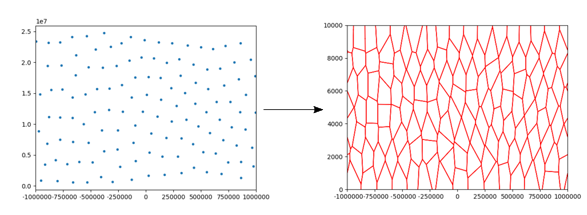
\includegraphics[width=\linewidth]{background/gpoints_mapping}
	\caption[Map from geostrophic points to fluid 'parcels']{Figure illustrating a map from geostrophic points to fluid 'parcels' that preserves volume.}
	\label{fig:gpointsmapping}
\end{figure}
The final piece is in the formulation of the solution of the semi-geostrophic equations as an optimal transport problem uses Theorem (3.16) from \cite{Cullen2006a}. We restate this using the notation above.
\begin{theorem}
	Given probability measures $\sigma$, $\mu$ with bounded supports $\Sigma \subset \mathbb{R}^2$, $\Gamma \subset \mathbb{R}^2 $. There exist optimal maps $t: \Sigma \rightarrow \Gamma$ and $t^{-1}: \Gamma \rightarrow \Sigma$ which are inverses and minimise a quadratic cost function given by
	\begin{equation*}
		\iint_{\mathbb{R}^2} \left(\frac{1}{2}f^2|\bm{Y}-t(\bm{Y})|^2\right)\sigma \ dXdZ
	\end{equation*}
	Furthermore, these maps are unique up to sets of measure zero.
\end{theorem}
The reader is referred to \cite{Rudin1987} for a detailed discussion of measure theory and zero measure sets.\\
\linebreak
The proof is given in \cite{Cullen2006a} and is a culmination of the results stated above. $\Gamma$ is clearly bounded by definition and $\Sigma$ is a set of finite points it too is also bounded. Furthermore since $sigma$ and $\mu$ are defined so that their integrals over $\Sigma$ and $\Gamma$ are unity, they are probability measures over their respective domains.
\\
\linebreak
It remains to show that the minimisation of the quadratic cost function is equivalent to minimising the energy. For this we transform the cost function to physical co-ordinates as,
\begin{equation*}
\iint_{\mathbb{R}^2} \left(\frac{1}{2}f^2|t^{-1}(\bm{y})-\bm{y}|^2\right) \ dxdz
\end{equation*}
The following Lemma proves this to be equivalent to minimising the energy given by \ref{energy}.
\begin{lemma}
	Minimising the Energy integral given by,
	\begin{equation*}
	E = f^2 \iint_{\Gamma} \frac{1}{2}\left(X-x\right)^2 - Z\left(z - H/2\right)\textrm{d}x\textrm{d}z
	\end{equation*} 
	is equivalent to minimising the quadratic cost integral given by,
	\begin{equation*}
	E = f^2 \iint_{\Gamma} \frac{1}{2}\left(\left(X-x\right)^2 + \left(Z - z\right)^2\right)\textrm{d}x\textrm{d}z
	\label{energy1}
	\end{equation*}
	\label{energy lemma}
\end{lemma}
\begin{proof}
	We begin by noting that the difference in the energy integrals is in the potential energy term, so it suffices to show that the minimisation of these terms is equivalent. Expanding to see,
	\begin{equation}
	\iint_{\Gamma} - Z\left(z - H/2\right)\textrm{d}x\textrm{d}z = \iint_{\Gamma} - Zz + \frac{ZH}{2}\textrm{d}x\textrm{d}z
	\label{min1}
	\end{equation} 
	\begin{equation}
	\iint_{\Gamma} \frac{1}{2}\left(Z - z\right)^2\textrm{d}x\textrm{d}z = \iint_{\Gamma} \frac{1}{2}Z^2 - Zz + \frac{1}{2} z^2 \ \textrm{d}x\textrm{d}z
	\label{min2}  
	\end{equation}
	Recalling that $Z$ is a function of $(x,z)$, the treatment of terms with this variable need to be considered carefully. As both \ref{min1} and \ref{min2} contain $\iint_{\Gamma} - Zz$, this can also be omitted from consideration.\\
	\linebreak
	Considering $\iint_{\Gamma} \frac{1}{2}Z^2\textrm{d}x\textrm{d}z$ . Given a partition of $\Gamma$ into $N$ cells up to zero measure sets, so that $\Gamma = \bigcup_{i=1}^N c_i$. Applying the transform $\Phi: (x,z) \rightarrow (X,Z)$, and using that the transform maps cells in physical space to points in geostrophic space
	\begin{equation*}
		\sum_{i=1}^N \iint_{c_i} \frac{1}{2}Z^2\textrm{d}x\textrm{d}z = \sum_{i=1}^N \iint_{\Phi(c_i)} \frac{1}{2}Z^2\sigma(X,Z) \ \textrm{d}X\textrm{d}Z 
	\end{equation*}
	But since $\sigma(X,Z) = \sum_{i=1}^{N} \frac{1}{N} \delta(\bm{Y}-\bm{Y_i})$
	\begin{equation*}
		\implies \sum_{i=1}^N \frac{1}{N} \frac{1}{2}Z_i^2
	\end{equation*}
	However this is a fixed value. Similar arguments give that,
	\begin{equation*}
		\sum_{i=1}^N \iint_{c_i} \frac{HZ}{2} \ \textrm{d}x\textrm{d}z = \sum_{i=1}^N \frac{HZ_i}{2}
	\end{equation*}
	Hence, the minimisation of \ref{min1} and \ref{min2} is equivalent.
\end{proof}
To summarise the results of this Chapter, we began by transforming the semi-geostrophic equations to geostrophic co-ordinates. In this setting finding the solution to equations \ref{EadyGC} was shown to amount to an energy minimisation problem with the energy being defined by \ref{energy}. Through the use of the Jacobian for the transformation $\sigma$ and an appropriately defined function $R(X,Z)$ we were able to show this energy minimisation to be the solution of a Monge Amp\'{e}re equation. Subsequently, through the use of probability measures this was shown to be equivalent to a discrte optimal transport problem with quadratic cost. Finally by showing the equivalence of minimising energy to minimising the quadratic cost function the problem is formulated as an optimal transport problem.
\comments{tie energy minimisation to Monge ampere equation/optimal transport}

%%%%%%%%%%%%%%%%%%%%%%%%%%%%%%%%%%%%%%%%%%%%%%%%%%%%%
\chapter{Semi-discrete Optimal Transport}
The Damped Newton algorithm, hereafter DA, developed by M\'{e}rigot et al. \cite{Merigot2017} solves a semi-discrete Monge-Amp\`{e}re type optimal transport problem. It's efficiency in exploiting the properties of sparse matrices and linear convergence \cite{Merigot2017} make it practical for implementation in the solution for equations \ref{EadyGC}. Further detail describing the application of the algorithm in the solution to the Eady Model is given in chapter \ref{algorithm}. In this chapter an overview of semi-discrete optimal transport is given using definitions given in \cite{Kitagawa2016, Merigot2017} as well as a comparison to the energy minimisation to which it is applied. A rigorous proof of the formulation of \ref{EadyModel} as a Monge-Amp\`{e}re type optimal transport problem is given in Cullen, 2006 \cite{Cullen2006a}.
\section{Semi-discrete Optimal Transport}
\begin{figure}[h]
	\centering
	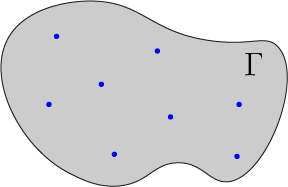
\includegraphics[width=5.5cm]{project/probmeasure}
	\caption[Semi-discrete Optimal Transport]{A discrete (target) set $Y \subseteq \mathbb{R}^2$ represented by blue points in a compact domain (source) $\Gamma \subseteq \mathbb{R}^2 $}
	\label{fig:probmeasure}
\end{figure}
Optimal transport problems describe the problem of finding a map between two sets, a target set and a source set, each with an associated density, in such a way that the "cost" associated with the mapping is minimised. In semi-discrete optimal transport the target set is a finite set.\\
\linebreak
In Kitagawa et al. \cite{Kitagawa2016} a wonderful analogy with travel distance to bakeries in a city is made, where the source set is considered as a city and the discrete target set is the locations of bakeries in the city. In this report the problem will be explained in the context in which it will subsequently be implemented. Namely, the source set is the domain $\Gamma$, the physical space described in section \ref{Chapter3} and the target set, the set of points in geostrophic space. The optimal transport problem finds a partition of the domain, up to sets of measure zero, such that every point in a region of the partion is closest to the point at the centre of that region. In this analogy the cost being minimised is the travel distance to the point $\bm{Y}_i$, $c(\bm{x},\bm{Y}_i) = \|\bm{x}-\bm{Y}_i \|^2$, where $\bm{x} \in \Gamma$. This is illustrated in figure \ref{fig:laguerrediagram0w}  below
\begin{figure}[h]
	\centering
	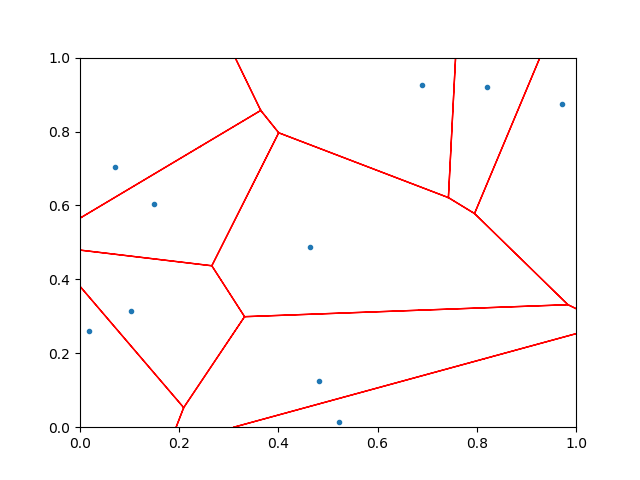
\includegraphics[width=8cm]{project/laguerre_diagram_0w}
	\caption[The partitioning of a Domain]{The image showing how a domain would be divided into areas based on minimising distance to the blue points. This is a Voronoi tesselation of the domain $\Gamma$ based on the minimisation of $c(\bm{x},\bm{Y_i})$}
	\label{fig:laguerrediagram0w}
\end{figure}
\\
To put this into a more rigorous mathematical setting, given a domain  $\Gamma\subseteq \mathbb{R}^2$ and discrete set of $N$ points $Y = \left\lbrace \bm{Y}_i = (X_i,Z_i), \quad 1\leq i \leq N \right\rbrace  \subset \mathbb{R}^2$,
\begin{definition}
	\textbf{Source measure} \\ Defined on the domain $\Gamma$. $\mu(A) = \textrm{Area}(\Gamma)^{-1}\int_A \ dxdz$, $A \subseteq \Gamma$. Note this defines a probability measure with a uniform probability density on $\Gamma$.
\end{definition}
\begin{definition}
	\textbf{Target measure} \\Defined on $\mathbb{R}^2$ $\sigma((X,Z)) = \sum_{i=1}^{N}\sigma_i \delta\left(\bm{Y}-\bm{Y}_i\right)$, with finite support on $\mathbb{R}^2$. Note this defines a discrete probability measure when $\sigma(\mathbb{R}^2) = 1$, for appropriate choice of $\sigma_i$.
	\label{target measure}
\end{definition}
\begin{definition}
	\textbf{Voronoi Cells} \\ The regions enclosed by the red lines and boundaries of the domain in \ref{fig:laguerrediagram0w} are defined as Voronoi cells, $\text{Vor}(\bm{Y}_i) := \left\lbrace \bm{x} \in \Gamma \; \text{st} \; \forall \ Y_j \in Y \; c(\bm{x},\bm{Y}_i) \leq c(\bm{x},\bm{Y}_j) \right\rbrace$. The diagram is referred to as a Voronoi tesselation.
\end{definition} 
\begin{definition} 
	\textbf{Transport map} \\ $T: \Gamma \rightarrow Y$ between the source measure $\mu$ and the target measure on $Y$, $\mu$ if $T_{\#}\mu = \sigma$.\\
\end{definition}
\begin{definition}
	\textbf{Pushforward} of a measure $\mu$ by a map $T: \Gamma \rightarrow Y$ is $T_{\#}\mu = \sum_{\bm{Y}_i \in Y} \mu \left( T^{-1}(\bm{Y}_i) \right) \delta(\bm{Y}-{\bm{Y}_i})$, the sum of the measures of the sets mapped to the points $\bm{Y}_i$ under $T$
\end{definition}
From these definitions we can see that the optimal transport map is given by,
\begin{equation}
	T(\bm{x}) = \arg\min_{\bm{Y}_i\in Y}\left(c(\bm{x},\bm{Y}_i)\right) \iff \sigma(\bm{Y}_i) = \mu\left(\text{Vor}(\bm{Y}_i)\right)
\end{equation}
\section{Laguerre Cells and the Inclusion of weights}
 \begin{figure}[h]
	\centering
	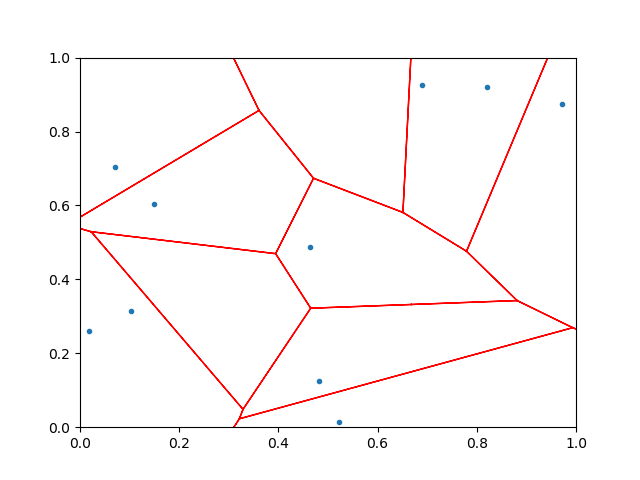
\includegraphics[width=8cm]{project/laguerre_diagram_OTw}
	\caption[Laguerre diagram produced by finding weights using DA for optimal transport]{Given a uniform source and target density the Laguerre diagram produced by finding weights using DA for optimal transport}
	\label{fig:laguerrediagramotw}
\end{figure}
Considering again figure \ref{fig:laguerrediagram0w} it is clear that if the density across the domain $\Gamma$ is uniform the distribution of area corresponding to each bakery is certainly not. For example, the Voronoi cells at the top right of the diagram in figure \ref{fig:laguerrediagram0w} are much larger in area than those in the centre of the diagram. This raises the problem of finding a way to create a partition such that each cell has the same area. This is done by introducing an additional$\ $\textquotedblleft weight\textquotedblright$\ $argument to the cost. We denote the weights by $\psi_i = \psi\left(\bm{Y}_i\right) \in \mathbb{R}$. In the case of the bakeries the weights might represent the price of bread at a specific bakery. For this we introduce the notion of Laguerre cells.\\
\begin{definition}
	\textbf{Laguerre Cells}\\
	 The regions enclosed by the red lines and boundaries of the domain in figure \ref{fig:laguerrediagramotw},  $\text{Lag}_{\bm{Y}_i}(\psi) := \left\lbrace \bm{x} \in \Gamma \; \text{st} \; \forall \ \bm{Y}_j \in Y \; c(\bm{x},\bm{Y}_i) + \psi(\bm{Y}_i) \leq c(\bm{x},\bm{Y}_j) + \psi(\bm{Y}_j) \right\rbrace$
	 \label{def: laguerre cell}
\end{definition}
In this case, the optimal transport map is given by \\
$T_\psi: x \rightarrow \text{argmin}_i\| x - y_i \|^2 + \psi_i$, where $\psi_i$ is a family of weights on $Y$ \cite{Merigot2017}.\\
\linebreak
 The problem is then finding the weights $\psi_i$ associated to the points $\bm{Y}_i$ such that $\mu (\text{Lag}_{\bm{Y}_i}(\psi)) = \sigma(\bm{Y}_i) = \sigma_i$. The Damped Newton's Algorithm from M\'{e}rigot, Meyron and Thibert (2017) \cite{Merigot2017} finds such $\psi_i$.
 \\
 \linebreak 
 Supposing that both the source density and target density are uniform, (ie) in definition \ref{target measure} the Laguerre cells as found by the DA code developed in \cite{Merigot2017} are shown in figure \ref{fig:laguerrediagramotw}. The Laguerre diagram highlights the fact that the densities are both specified to be uniform probability densities. In figure \ref{fig:laguerrediagram0w} the target density was not specified. This means that points are not necessarily interior to their corresponding Laguerre cells, however the cells have equal area. The cells in this case are the Laguerre cells defined above, and the weights that define the optimal transport map was found by \cite{Merigot2017} as
 \begin{equation*}
 T(x) = \arg\min_{\bm{Y}_i\in Y}\left(c(\bm{x},\bm{Y}_i) + \psi_i\right)
 \end{equation*}
For the remainder of this report we will consider cases where both the source density and target density are uniform and the quadratic cost function is,
\begin{equation*}
	c(\bm{x},\bm{Y}_i) = \| \bm{x} - \bm{Y}_i \|^2
\end{equation*}
\section{Applying semi-discrete optimal transport to solving the semi-geostrophic equations}
As shown in \cite{Cullen2006a} equations \ref{EadyModel} can be recast as an optimal transport problem using the transformation to geostrophic co-ordinates introduced by Hoskins \cite{Hoskins1975}. In this section we outline how DA is applied to equations \ref{EadyModel}.
\\
\linebreak
The optimal transport problem considered in the frontogenesis problem is the minimisation of the energy, restated from equation \ref{energy}
\begin{equation}
E = f^2 \iint \frac{1}{2}\left(X-x\right)^2 - Z\left(z - H/2\right)\textrm{d}x\textrm{d}z
\end{equation}
as shown by Lemma \ref{energy lemma} this is equivalent to minimising \ref{energy1},
\begin{equation}
E = \frac{f^2}{2} \iint \left(\left(X-x\right)^2 + \left(Z - z\right)^2\right)\textrm{d}x\textrm{d}z
\end{equation}
Considering the geostrophic co-ordinates as the target set of finite set of points for the optimal transport problem from the domain $\Gamma = [-L,L] \times [0,H]$. The DA Algorithm finds the weights such that the area of each Laguerre cell is preserved. Physically, this amounts to the condition that the volume is conserved.
\section{Extension for Periodic Boundary Conditions}
As stated in Chapter \ref{governingequations} in the model for frontogenesis boundary conditions consider periodicity in $x$. This must be accounted for in the implementation of the Damped Newton Algorithm.
\\
\linebreak
This inclusion of periodic boundary conditions allows Laguerre cells to cover areas over the right and left boundaries. This means that the Laguerre edges must be continuous across the boundaries if copies of the Laguerre diagram were placed on each boundary. The Laguerre cells must have the same mass, for example, in figure \ref{fig:laguerrediagramotpw} below the top right cell extends to the left of the domain. The sum of the areas of each component of the cell must be the same as a cell in the centre of the diagram. The area of each cell remains the same as in \ref{fig:laguerrediagramotw} however the boundaries of the Laguerre cells are continuous across the left and right boundaries of the domain.
\begin{figure}[h]
	\centering
	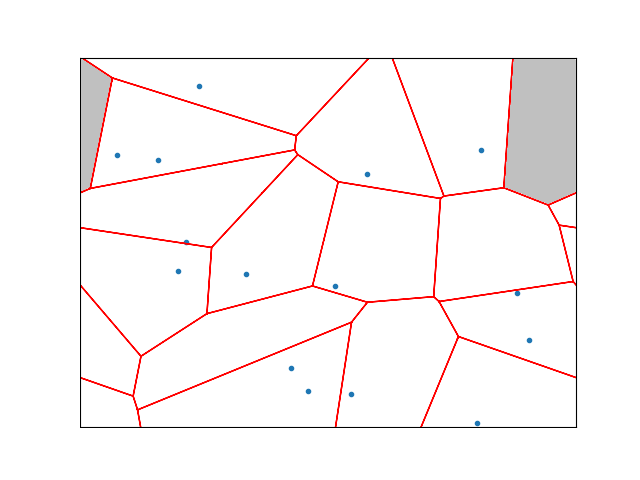
\includegraphics[width=8cm]{project/laguerre_diagram_OTPw}
	\caption[Optimal Transport with Periodic Boundary Conditions]{The solution to the optimal transport of the same points shown in figure \ref{fig:laguerrediagramotw}, however with the density initialised with periodic boundary conditions in $x$. The area shaded in grey represents a single Laguerre cell.}
	\label{fig:laguerrediagramotpw}
\end{figure}
\subsection{Definitions of Mass with Periodic Boundary Conditions}
\begin{figure}[h]
	\centering
	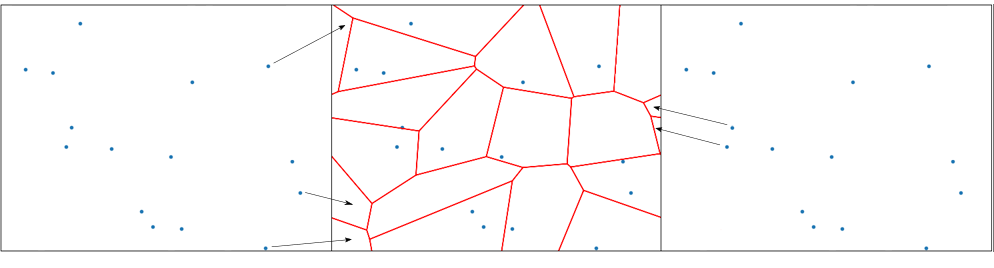
\includegraphics[width=1\linewidth]{project/laguerre_diagram_OTPw_periodic}
	\caption[Periodic boundary conditions with 'ghost' points]{The image above shows how the Laguerre diagram for periodic boundary conditions is created with 'ghost' points on either side of the domain. Arrows show where ghost points contribute to Laguerre cells of positive mass in the domain $\Gamma$}
\end{figure}

\comments{include the definition of mass of a cell and a better written description of the partition given by a laguerre diagram (tesselation/zero measure sets)}
\comments{include definition of the fundamental domain}
\subsection{Mapping to the Fundamental Domain}
Under the geostrophic transformation \ref{transformation} and also in time-stepping points in geostrophic space it is possible for points to travel exterior the boundaries of the domain $\Gamma$. In the $x$ direction the boundary conditions imposed are periodic. If points are mapped so that their $x$-co-ordinates are exterior to the interval $[-L,L]$, they can be mapped to the domain $\Gamma$, the \textquoteleft fundamental domain\textquoteright, using the periodicity, without affecting the result. \comments{better phrasing please} In fact, in the implementation of DA this is necessary at every time step to ensure that the mass of cells remains positive. This is implemented by the function \textquoteleft to\_fundamental\_domain\textquoteright \ adapted from DA \cite{Merigot2017a} to treat periodic boundary conditions in $x$. An example of this is shown in figure \ref{fundamental domain} below, where the fundamental domain being considered is $[0,1]\times[0,1]$.
\begin{figure}[h!]
	\centering
	\subfloat[]{{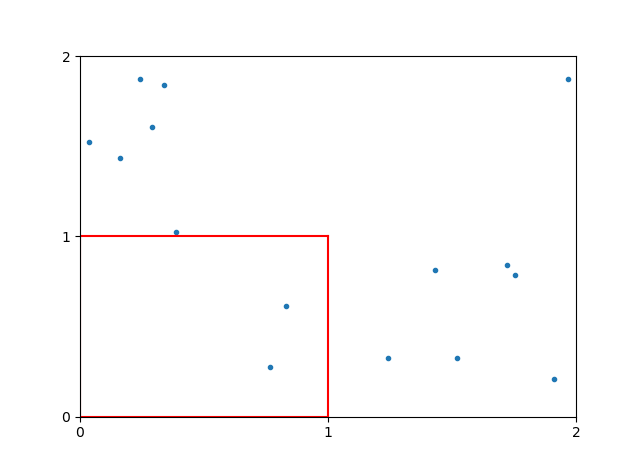
\includegraphics[width=7cm]{project/fund_domain_out}\label{out of fund domain}}}
	\subfloat[]{{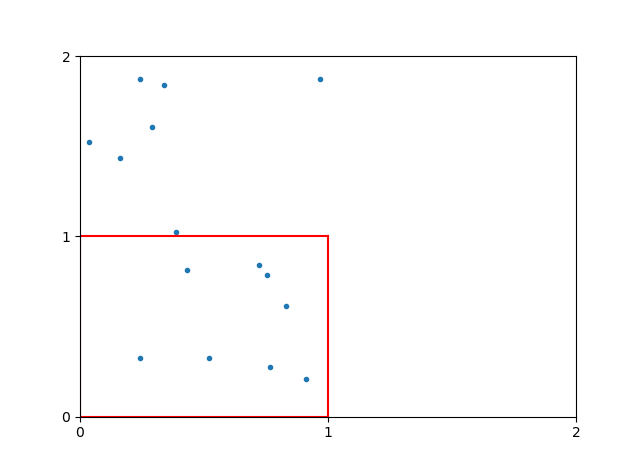
\includegraphics[width=7cm]{project/fund_domain_in}\label{in fund domain}}}
	\caption{Plots of a random set of points initialised in $[0,2]\times[0,2]$ before (a) and after (b) being mapped to the fundamental domain $[0,1]\times[0,1]$}
	\label{fundamental domain}
\end{figure}
\\
To explain this rigorously, we consider the domain described by $[x_0,y_0] \times [x_1,y_1]$. Since we are only considering periodic boundary conditions in $x$, only the $x$ co-ordinates will be mapped. 
\\
The mapping is performed by first finding the distance of the point from the left boundary of the domain as a ratio of the width of the domain. This is then added to left bound to give a value for $x$, $\tilde{x}$ that is in the fundamental domain. 
\begin{equation*}
	\begin{aligned}
		X &= x - \floor*{\frac{x - x_0}{x_1 - x_0}}\\
		\tilde{x} &= x_0 + (x_1 - x_0)X
	\end{aligned}
\end{equation*}
This is implemented as:
\comments{insert to\_fundamental\_domain code}
%%%%%%%%%%%%%%%%%%%%%%%%%%%%%%%%%%%%%%%%%%%%%%%%%%%%%
\chapter{A Numerical Solution to the Eady Model for Frontogenesis \label{algorithm}}
In this section the numerical implementation including the use of the Damped Newton Algroithm developed by \cite{Merigot2017} is explained in detail. 
Restating the problem, we are solving the semi-geostrophic equations \ref{EadyModel} over the domain $\Gamma := [-L,L] \times [0,H]$.
\begin{equation*}
	\begin{aligned}
		-fv_g + \frac{\partial \varphi}{\partial x} = 0,\\
		\frac{Dv_g}{Dt} + fu -\frac{Cg}{\theta _0}\left(z-H/2\right) = 0,\\
		\frac{D\theta'}{Dt} - Cv_g = 0,\\
		\frac{\partial \varphi}{\partial z} - g\frac{\theta'}{\theta_0} = 0,\\
		\nabla \cdot \bm{u} = 0.
	\end{aligned}
\end{equation*}
With boundary conditions:
\vspace{-\topsep}
\begin{itemize}
	\setlength{\parskip}{0pt}
	\setlength{\itemsep}{0pt}
	\item Rigid lid condition $w = 0$ on $z = 0, H$
	\item Periodic boundary conditions in $x$
\end{itemize}
\vspace{-\topsep}
Together with a baroclinic instability described by \ref{thetap} as
\begin{equation}
\theta' = \frac{N^2\theta_0 z}{g} + B\sin\left(\pi\left(x/L + z/H\right)\right)
\end{equation}
The steps involved in solving the Eady Model for frontogenesis described above are detailed below,
\begin{description}
	\setlength{\parskip}{0pt}
	\setlength{\itemsep}{0pt}
	\item[Step 1] Initialise a set of points in physical space
	\item[Step 2] Transform physical points to Geostrophic space using the co-ordinate transformation given in \ref{transformation}, and map to fundamental domain $\Gamma$.
	\item[Step 3] Given the points in geostrophic space the weights which define the Laguerre cells in the physical domain are calculated using the Damped Newton Algorithm.
	\item[Step 4] The equations are now time stepped from the transformed momentum equations \ref{EadyGC} 
	\begin{equation*}
		\begin{aligned}
			\frac{\mathrm{D}X_{n}}{\mathrm{D}t} -\frac{Cg}{f\theta _0}\left(\tilde{z}_n-H/2\right) = 0 \\
			\frac{\mathrm{D}Z_{n}}{\mathrm{D}t} - \frac{Cg}{f\theta_0}\left(X_n - \tilde{x}_n\right) = 0
		\end{aligned}
	\end{equation*}
	Where $X_n, Z_n$ represent the geostrophic points at the current time step, and $\tilde{x}_n,\tilde{z}_n$ represent the centroids of the Laguerre cells. In this project both a Forward-Euler scheme and Heun's method have been used for time-stepping.
	\item[Step 5] The geostrophic points are now replaced with $X_{n+1}, Z_{n+1}$ and steps 3 and 4 are repeated until the final time is reached.
\end{description}
\section{Initialisation of Points in Geostrophic Space \label{Initpoints}}
Given a finite set of equidistant points in the physical domain $\Gamma$, the points are transformed to geostrophic space using
\begin{equation}
X = x + \frac{v_g}{f}, \qquad Z = \frac{g\theta'}{f^2\theta_0}
\label{geostrophictransformation}
\end{equation}
This requires the form of $\theta'$ given by \ref{thetap} from this $v_g$ can be deduced using the following equations from \ref{EadyModel},
\begin{equation}
	\begin{aligned}
		\frac{\partial \varphi}{\partial z} - \frac{g \theta'}{\theta_0} = 0\\
		\frac{\partial \varphi}{\partial x} - fv_g = 0
	\end{aligned}
\label{findingvg}
\end{equation}
using the boundary condition $\int_{0}^{H}\varphi(x,z)\text{ d}z = 0$
Integrating the first equation in $z$,
\begin{equation*}
	\begin{aligned}
	\frac{\partial \varphi}{\partial z} = \frac{g \theta'}{\theta_0} = N_0^2z + \frac{Bg}{\theta_0}\sin\left(\pi\left(\frac{x}{L}+\frac{z}{H}\right) \right)\\
	\varphi = \frac{N_0^2z^2}{2} - \frac{BgH}{\theta_0\pi}\cos\left(\pi\left(\frac{x}{L}+\frac{z}{H}\right)\right) + F(x)
	\end{aligned}
\end{equation*}
Applying the boundary condition to determine $F(x)$,
\begin{equation*}
	\begin{aligned}
	\int_{0}^{H}\varphi \text{ d}z = \left[ \frac{N_0^2z^3}{6} - \frac{BgH^2}{\theta_0\pi^2}\sin\left(\pi\left(\frac{x}{L}+\frac{z}{H}\right) \right) + F(x)z\right]_{0}^{H} = 0
	\end{aligned}
\end{equation*}
Using $\sin\left(\frac{\pi x}{L}+\pi\right) = -\sin\left(\frac{\pi x}{L}\right)$,
\begin{equation*}
\begin{aligned}
 0 & =\frac{N_0^2H^3}{6} - \frac{BgH^2}{\theta_0\pi^2}\sin\left(\frac{\pi x}{L}+\pi\right)+ \frac{BgH^2}{\theta_0\pi^2}\sin\left(\frac{\pi x}{L}\right) + F(x)H\\
 0 & =\frac{N_0^2H^3}{6} + \frac{2BgH^2}{\theta_0\pi^2}\sin\left(\frac{\pi x}{L}\right) + F(x)H
\end{aligned}
\end{equation*}
This gives $F(x)$ as,
\begin{equation*}
	F(x) = -\frac{N_0^2H^2}{6} - \frac{2BgH^2}{\theta_0\pi^2}\sin\left(\frac{\pi x}{L}\right)
\end{equation*}
and consequently $\varphi$ as,
\begin{equation}
	\varphi(x,z) = \frac{N_0^2z^2}{2} - \frac{BgH}{\theta_0\pi}\cos\left(\pi\left(\frac{x}{L}+\frac{z}{H}\right)\right)-\frac{N_0^2H^2}{6} - \frac{2BgH}{\theta_0\pi^2}\sin\left(\frac{\pi x}{L}\right)
\end{equation}
Using the second of equations \ref{findingvg} $v_g$ is found as,
\begin{equation}
	v_g = \frac{BgH}{f\theta_0L}\cos\left(\pi\left(\frac{x}{L}+\frac{z}{H}\right)\right)- \frac{2BgH}{f\theta_0\pi}\sin\left(\frac{\pi x}{L}\right)
	\label{vg}
\end{equation}
Together with $\theta'$ given by \ref{thetap} this expression for $v_g$ can be used to determine $X$ and $Z$ in geostrophic co-ordinates through the transform \ref{geostrophictransformation}.
\begin{figure}[h]
	\centering
	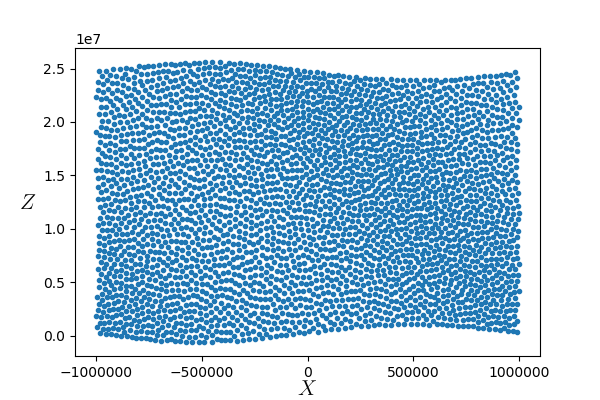
\includegraphics[width=7cm]{project/gpoints}
	\caption[Plot of Points in Geostrophic Space]{Plot of points in geostrophic space, transformed from a random set of points in $\Gamma := [-L,L] \times [0,H]$ using \ref{transformation} with $v_g$ as defined in \ref{vg}}
	\label{fig:gpoints}
\end{figure}

\section{Choice of Initial Weights \label{Initweights}}
The Laguerre diagram of this set of points shown in figure \ref{fig:gpoints} with zero weights would define Laguerre cells exterior to $\Gamma$. These cells will have zero \textquotedblleft mass \textquotedblright in the domain $\Gamma$. Physical intuition tells us that given the rigid lid and periodic boundary conditions points would physically not be able to leave the domain. However, thinking of fluid particles as the centroids of Laguerre cells, a cell outside the domain would represent a fluid particle on the exterior of the domain. This also poses a problem with respect to the implementation of DA, as emphasised in \cite{Merigot2017}, as it requires $\mu\left(\text{Lag}_{y_i}(\psi)\right)$ to be a monotonic function of $\psi = (\psi(y_1),...,\psi(y_N))$ where $N$ is the number of points initialised in $\Gamma$. According to \cite{Merigot2017} this occurs near points where the Laguerre cells contain positive mass over $\Gamma$.\\
\linebreak
Fortunately, a solution is provided in \cite{Merigot2017}. Proposition 25 in the paper proves that if the initial weights are given by,
\begin{equation*}
	\psi_i^0 = d\left(\bm{Y}_i,\Gamma\right)^2
\end{equation*}
where $\bm{Y}_i = \left(X_i,Z_i\right)$ are the points in geostrophic space. Since the domain is rectangular vertical distance from the point to the upper or lower boundary of the domain. The boundaries, given by $z=0$ and $z = H$ are also perturbed to guarantee strict positivity of the mass of the Laguerre cells, 
\begin{equation}
\psi_i^0 = \begin{cases}
\left(Z_i - 0.9H\right)^2, & Z_i > 0.9H \\
\left(Z_i - 0.1H\right)^2, & Z_i < 0.1H
\end{cases}
\label{weights}
\end{equation}
\comments{Address disparity with paper '-' sign - convention used in paper for finding Laguerre cells different to code?}
The Damped newton algorithm, DA, is initialised with the the geostrophic points and weights given by \ref{weights}. The algorithm outputs weights that give Laguerre cells with equal mass over the periodic domain.
\section{Time Stepping \label{timestep}}
Once the initial points and weights have been set up, it remains to find the geostrophic points at the next time step, using equations \ref{EadyGC}.
\subsection{Forward-Euler Scheme}
The numerical solution to equations \ref{EadyModel} developed follows a Lagrangian framework, thus it is justified to treat the material derivative $\frac{\mathrm{D } }{\mathrm{D} t}$ as a full derivative $\frac{\mathrm{d }}{\mathrm{d} t}$, in this sense we will develop prognostic scheme using the equations,
	\begin{equation*}
	\begin{aligned}
	\frac{\mathrm{d}X}{\mathrm{d}t} -\frac{Cg}{f\theta _0}\left(\tilde{z}-H/2\right) = 0 \\
	\frac{\mathrm{d}Z}{\mathrm{d}t} - \frac{Cg}{f\theta_0}\left(X - \tilde{x}\right) = 0
	\end{aligned}
	\end{equation*}
Applying a Forward-Euler scheme \cite{Griffiths2010} for time-stepping given by,
\begin{equation}
	\begin{aligned}
	t^{n+1} &= t^n + h\\
	Z_i^{n+1} &= Z_i^n + \frac{hCg}{f\theta_0}\left(X_i^n-\tilde{x}_i^n\right)\\
	X_i^{n+1} &= X_i^n + \frac{hCg}{f\theta_0}\left(\tilde{z}_i^n-H/2\right)
	\end{aligned}
\end{equation}
where $\tilde{x}_i^n,\tilde{z}_i^n$ represent the centroids of the Laguerre cells given by equations \ref{centroids} using $X_i^n,Z_i^n$ and corresponding weights given by the optimal transport algorithm (DA),
\begin{equation}
	\tilde{x}_i^n = \frac{\int_{\mathrm{Lag}_{\bm{Y}_i^n}(\psi)} x \  \mathrm{d}x \mathrm{d}z}{\int_{\mathrm{Lag}_{\bm{Y}_i^n}(\psi)} \mathrm{d}x \mathrm{d}z}, \qquad
	\tilde{z}_i^n = \frac{\int_{\mathrm{Lag}_{\bm{Y}_i^n}(\psi)} z \ \mathrm{d}x \mathrm{d}z}{\int_{\mathrm{Lag}_{\bm{Y}_i^n}(\psi)} \mathrm{d}x \mathrm{d}z}
	\label{centroids}
\end{equation}
Before the next iteration of the time-step the points $X_i^{n+1}, Z_i^{n+1}$ are mapped back to the fundamental domain.
\subsection{Heun's Method}
For comparison and to test convergence the time-stepping was also implemented using Heun's method \cite{Griffiths2010}.
\begin{equation}
	\begin{aligned}
	t^{n+1} &= t^{n} + h, \quad
	\hat{Z}_i^{n+1} = Z_i^n +  \frac{hCg}{f\theta_0}\left(X_i^n-\tilde{x}_i^n\right), \quad
	\hat{X}_i^{n+1}  = X_i^n +  \frac{hCg}{f\theta_0}\left(\tilde{z}_i^n-H/2\right)\\
	Z_i^{n+1} &= Z_i^n + \frac{h}{2}\left( \frac{Cg}{f\theta_0}\left(X_i^n-\tilde{x}_i^n\right)+ \frac{Cg}{f\theta_0}\left(\hat{X}_i^{n+1}-\hat{x}_i^{n+1}\right)\right)\\
	X_i^{n+1}  &= X_i^n + \frac{h}{2}\left( \frac{Cg}{f\theta_0}\left(\tilde{z}_i^n-H/2\right) + \frac{Cg}{f\theta_0}\left(\hat{z}_i^{n+1}-H/2\right)\right)
	\end{aligned}
\end{equation}
Where again, $\hat{x}_i^n$ and $\hat{z}_i^n$ represent the centroids of the Laguerre cells given using \ref{centroids} and $\hat{X}_i^{n+1},\hat{Z}_i^{n+1}$ with corresponding weights given by the optimal transport algorithm DA.

\comments{why not higher order time-step method? Limited by OT solver - 2nd order?}
\comments{include map back to fundamental domain explanation and why this isn't done for centroids}
A comparison of results using Heun's method and the forward-Euler scheme for timestepping is detailed in Chapter \ref{results}.
\section{Visualising the Output \label{plotting}}
Given the Geostrophic points and the associated weights which solve the optimal transport problem a Laguerre diagram satisfying \ref{def: laguerre cell} can be constructed. In the Monge-Amp\`{e}re library of DA \cite{Merigot2017,Merigot2017a} there is a function to rasterize a Laguerre diagram to a pixelated image, with Laguerre cells coloured according to the value of a particular variable.\\
\linebreak
For example, in the images below the Laguerre cells are coloured according to the value of $\theta '$ given by, $\theta ' = \frac{f^2\theta_0 Z}{g}$
%%%%%%%%%%%%%%%%%%%%%%%%%%%%%%%%%%%%%%%%%%%%%%%%%%%%%

\chapter{Numerical Simulations and Results \label{results}}
In this chapter we discuss the numerical results of the implementation of algorithm \ref{Algorithm} using the PyMongeAmpere library \cite{Merigot2017a} for solving the optimal transport problem. The use of this algorithm allows us to produce results with higher resolutions than previously realised. Plotting the Laguerre diagrams confirms the formation of a front as compared to similar results produced by \cite{Nakamura1994,Cullen1993}. Finally, the validity of the numerical implementation is investigated and performance analysed to assert the suitability of the numerical implementation in providing a solution to equations \ref{EadyModel}.
\section{Physical interpretation of Results \label{laguerre plots}}
Using the plotting process described in section \ref{plotting}. The Laguerre diagrams below show snapshots of frontogenesis and the subsequent evolution of the front. The model was initialised with a grid of $80 \times 40$ points taken from an optimised sampling of points in the physical domain $\Gamma = [-L,L]\times[0,H]$ and transformed to geostrophic co-ordinates as explained in \ref{Initpoints}. This involves an application of Lloyd's algorithm where first moments of cells are iteratively found until points are equidistant in the domain. A summary of parameter values in given in table \ref{param vals}.  For the following results Heun's method described in section \ref{Heun} was used for time-stepping for a time period of 25 days from a randomly generated mesh.
\\
\linebreak
\begin{table}
	\begin{tabular}{|c|c|c|c|}
		\hline 
		Parameter & Value & Parameter & Value \\
		\hline 
		$L$ & $1 \times 10^6 \ m$ & $H$ & $1 \times 10^4 \ m$ \\ 
		\hline 
		$g$ & $10 \ ms^{-2}$ &	$f$ & $10^{-4} \ s^{-1}$ \\ 
		\hline 
		$N^2$ & $2.5 \times10^{-5} \ s^{-2}$&$\theta_0$ & $300 \ K$ \\ 
		\hline 
		C & $3 \times 10^{-6} \ m^{-1}K$ & $B$ & $0.25 \ Ks^{-1}$ \\ 
		\hline 
	\end{tabular}
	\caption[Table of parameter values used in numerical implementation of SG/DA]{Table of parameter values used in numerical implementation of SG/DA as given by \cite{Cullen2006a} with $B$ chosen independently.}
	\label{param vals}
\end{table}
In diagrams \ref{fig: thetap ldiag1}-\ref{fig: thetap ldiag2} we see the growth of the normal mode instability. Initially (a) the stratification of potential temperature, $\theta '$ is linear, as in the base state. By $2.5$ (b) days we see the instability appear in the form of a wave and by $6$ days a strong front has formed as a large gradient in $\theta '$. We see that warmer air in the upper atmosphere has been come down into the lower regions of the atmosphere. By (d) the front has collapsed again as the normal mode instability loses its predominance. 
\\
\linebreak
An interesting phenomenon observed after this is that the instability grows again and a secondary front is formed. A cycle then forms of an growing instability in one direction forming a front which is then dissipated and a subsequent instability grows in the opposite direction. Some snapshots of this cycle are shown in the images below. This cycle is due to the balance between the normal mode instability and the background shear. Initially the instability is free to grow dominating the dynamics and leading to frontogenesis. The vertical shear counterbalances the growth of the instability dissipating the front. Internal instabilities then act to contribute towards the growth of a new front, however this secondary front is not as strong. The vertical shear again acts to restore the system to its original state and the cycle continues like this. 
\newpage
\begin{figure}[ht!]
	\centering
	\subfloat[]{{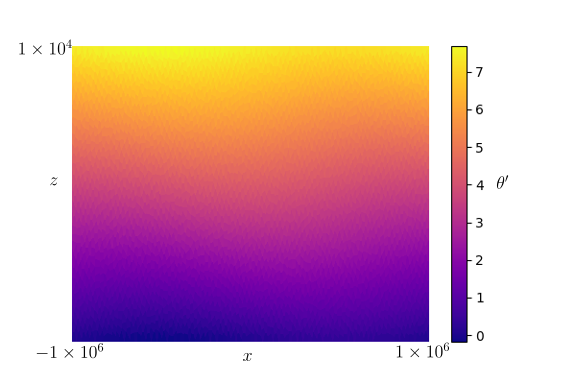
\includegraphics[width=0.9\linewidth]{evaluation/laguerre_diagram_thetap_0}}}\\
	\subfloat[]{{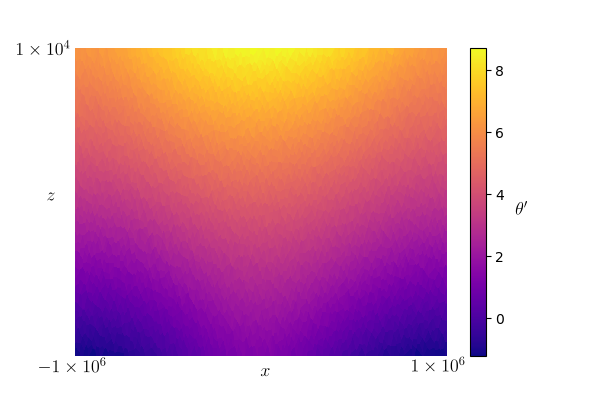
\includegraphics[width=0.9\linewidth]{evaluation/laguerre_diagram_thetap_5}}}
	\caption{Plots of Laguerre Diagrams shaded according to the value of $\theta '$ using a random mesh of $80 \times 40$ points initialised in geostrophic space using \ref{Initpoints} at (a) $0$ days, (b) $2.5$ days (c) $6$ days and (d) $9$ days, $\Gamma = [-L,L]\times[0,H]$, where $L = 1\times10^6$ and $H = 1\times10^4$}
	\label{fig: thetap ldiag1}
\end{figure}
\begin{figure}[ht!]
	\centering
	\subfloat[]{{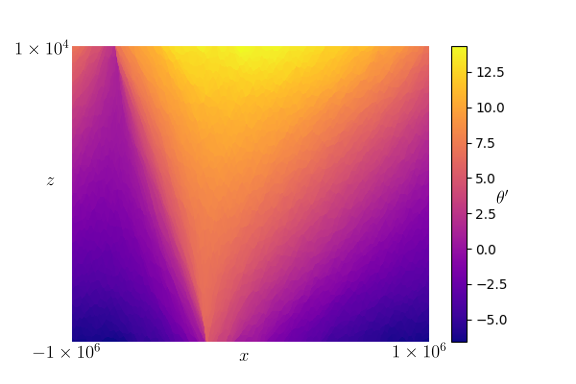
\includegraphics[width=0.9\linewidth]{evaluation/laguerre_diagram_thetap_12}}}\\
	\subfloat[]{{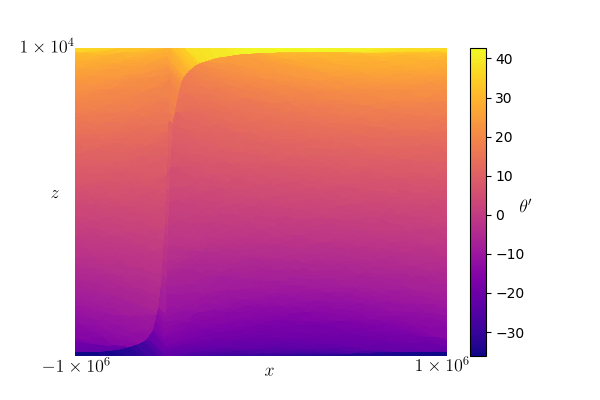
\includegraphics[width=0.9\linewidth]{evaluation/laguerre_diagram_thetap_18}}}\\
	\caption{Plots of Laguerre Diagrams shaded according to the value of $\theta '$ using a random mesh of $80 \times 40$ points initialised in geostrophic space using \ref{Initpoints} at (a) $6$ days, (b) $9$ days, $\Gamma = [-L,L]\times[0,H]$, where $L = 1\times10^6$ and $H = 1\times10^4$}
	\label{fig: thetap ldiag2}
\end{figure}
\newpage
Diagram (a) in \ref{fig: front_cycle} shows the formation of the secondary front, (b) \ref{fig: front_cycle}  in  shows its collapse and (c) shows the formation of a third front with a reversed gradient in $\theta '$. The front formation is not as clear in these images. The range in $\theta '$ has been reduced to half its original range to illustrate the cycle better. This leads to a saturation of colour at the top an bottom of the Laguerre diagrams as extreme values of $\theta '$ are mapped to the end points of the scale. As suggested by Dr Cotter this could be due to outlying points which contribute to extreme values of $\theta '$. This skews the colour range as seen in figure \ref{fig: front_cycle}
\begin{figure}[h!]
	\centering
	\subfloat[]{{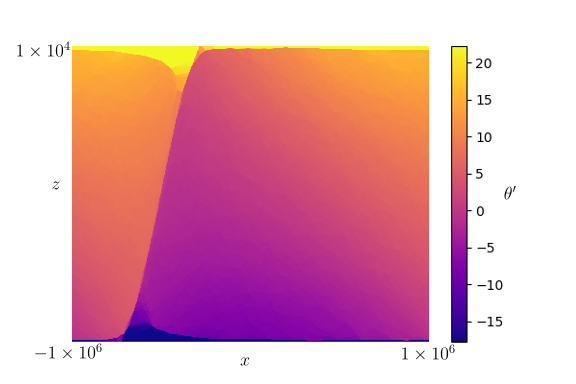
\includegraphics[width=0.6\linewidth]{evaluation/laguerre_diagram_thetap_22}}}\\
	\subfloat[]{{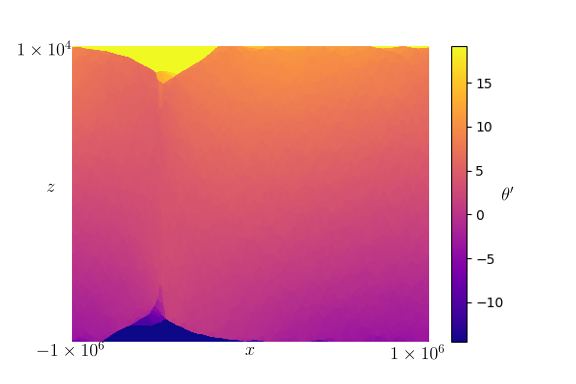
\includegraphics[width=0.6\linewidth]{evaluation/laguerre_diagram_thetap_25}}}\\
	\subfloat[]{{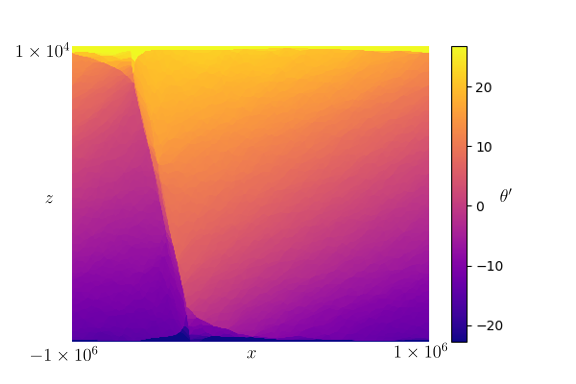
\includegraphics[width=0.6\linewidth]{evaluation/laguerre_diagram_thetap_29}}}\\
	\caption{Plots of Laguerre Diagrams shaded according to the value of $\theta '$ using a random mesh of $80 \times 40$ points initialised in geostrophic space using \ref{Initpoints} at (a) $11$ days, (b) $12.5$ days (c) $14.5$ days, $\Gamma = [-L,L]\times[0,H]$, where $L = 1\times10^6$ and $H = 1\times10^4$}
	\label{fig: front_cycle}
\end{figure}


\begin{figure}[ht!]
	\centering
	\subfloat[]{{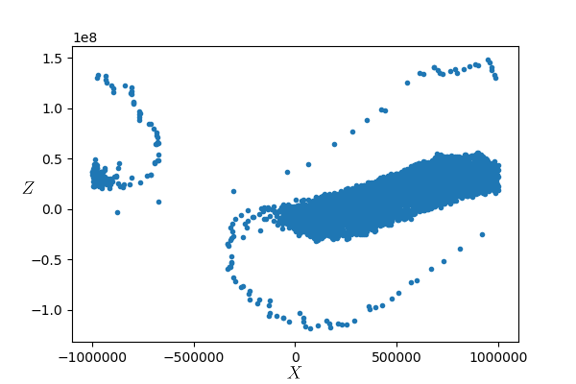
\includegraphics[width=0.6\linewidth]{evaluation/Gpoints_22}}\label{Gpoints_front11}}
	\caption{Plot of Geostrophic points at $11$ days}
	\subfloat[]{{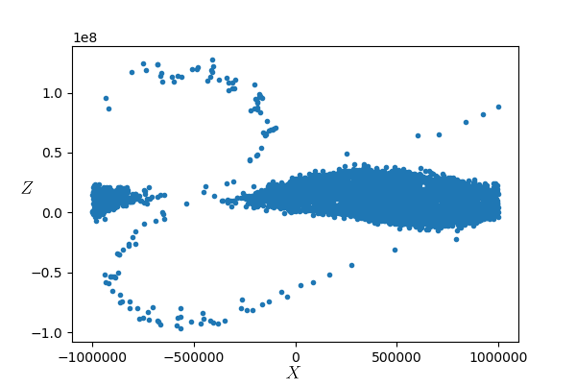
\includegraphics[width=0.6\linewidth]{evaluation/Gpoints_25}}\label{Gpoints_front12.5}}
	\caption{Plot of Geostrophic points at $12.5$ days}
	\subfloat[]{{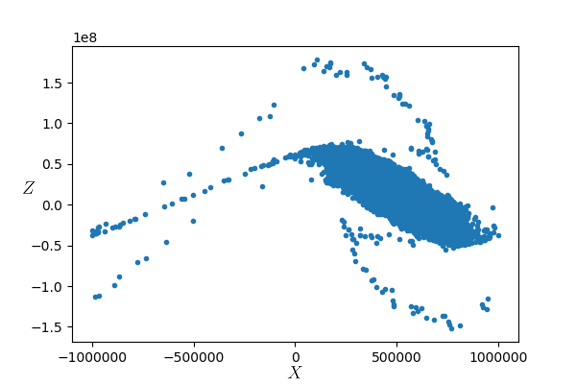
\includegraphics[width=0.6\linewidth]{evaluation/Gpoints_29}}\label{Gpoints_front14.5}}
	\caption{Plot of Geostrophic points at $14.5$ days}
\end{figure}

Another interesting visualisation of the result is that of using $v_g$ the cross slice velocity as a colour scale. The diagrams below illustrate this for the same data as in figures \ref{fig: thetap ldiag1}, \ref{fig: thetap ldiag2}. The front formation is a lot clearer in this case especially for the cycle of front formation and collapse.
\newpage
\begin{figure}[ht!]
	\centering
	\subfloat[]{{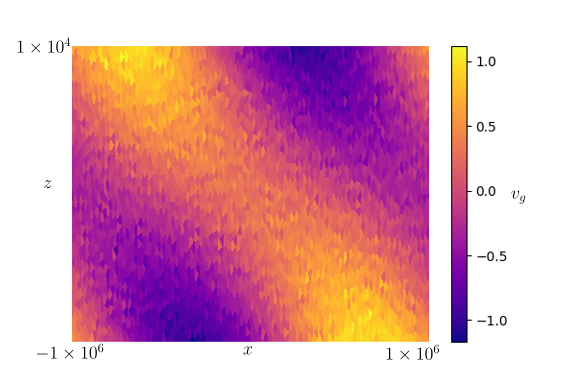
\includegraphics[width=0.7\linewidth]{evaluation/laguerre_diagram_vg_0}}}\\
	\subfloat[]{{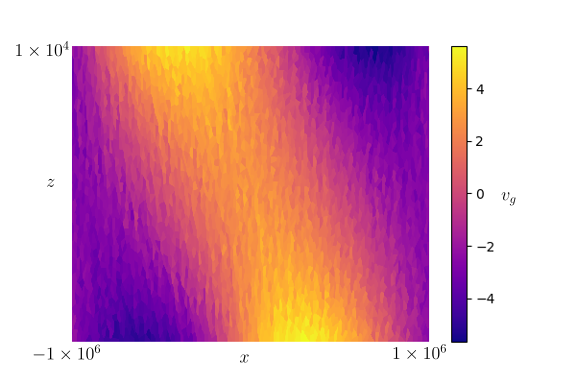
\includegraphics[width=0.7\linewidth]{evaluation/laguerre_diagram_vg_5}}}
	\caption{Plot of Laguerre Diagrams shaded according to the value of $v_g$ using a random mesh of $80 \times 40$ points initialised in geostrophic space using \ref{Initpoints} at (a) $0$ days and (b) $2.5$ days , $\Gamma = [-L,L]\times[0,H]$, where $L = 1\times10^6$ and $H = 1\times10^4$}
	\label{vg0}
\end{figure}
\newpage
\begin{figure}[h!]
	\centering
	\subfloat[]{{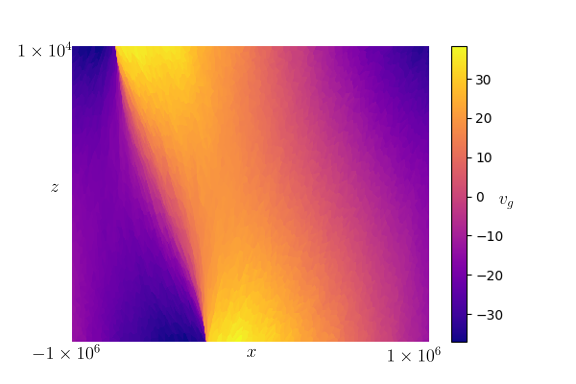
\includegraphics[width=0.7\linewidth]{evaluation/laguerre_diagram_vg_12}}}\\
	\subfloat[]{{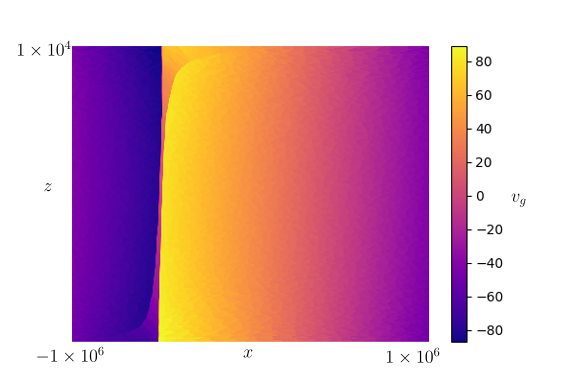
\includegraphics[width=0.7\linewidth]{evaluation/laguerre_diagram_vg_18}}}
	\caption{Plots of Laguerre Diagrams shaded according to the value of $v_g$ using a random mesh of $80 \times 40$ points initialised in geostrophic space using \ref{Initpoints} at (a) $6$ days (b) $9$ days $\Gamma = [-L,L]\times[0,H]$, where $L = 1\times10^6$ and $H = 1\times10^4$}
	\label{vg2.5}
\end{figure}
\begin{figure}[ht!]
	\centering
	\subfloat[]{{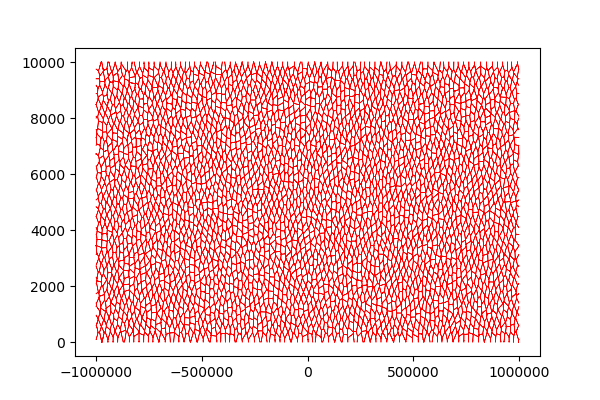
\includegraphics[width=0.7\linewidth]{evaluation/laguerre_tesselation_0}}}\\
	\subfloat[]{{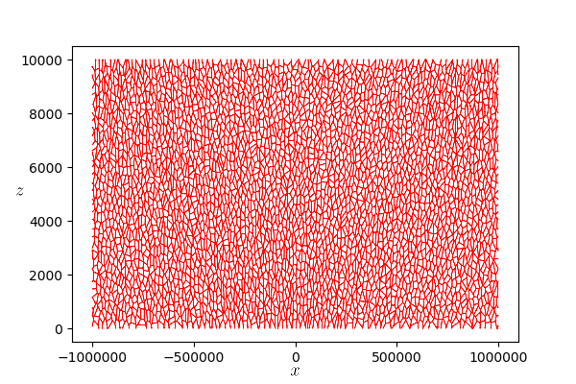
\includegraphics[width=0.7\linewidth]{evaluation/laguerre_tesselation_5}}}
	\caption{Plot of Laguerre Cells generated using a random mesh of $80 \times 40$ points initialised in geostrophic space using \ref{Initpoints} at (a) $0$ days and (b) $2.5$ days , $\Gamma = [-L,L]\times[0,H]$, where $L = 1\times10^6$ and $H = 1\times10^4$}
	\label{lagcells1}
\end{figure}
\newpage
\begin{figure}[h!]
	\centering
	\subfloat[]{{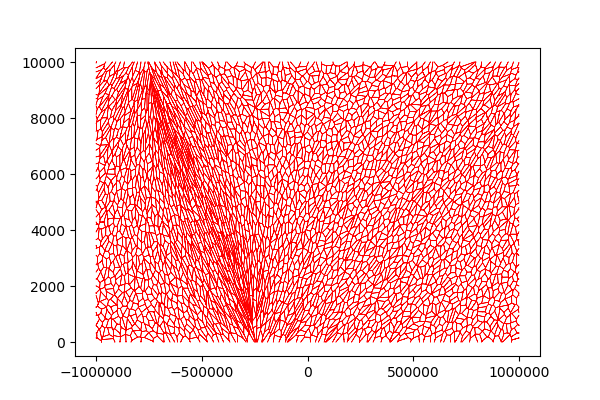
\includegraphics[width=0.7\linewidth]{evaluation/laguerre_tesselation_12}}}\\
	\subfloat[]{{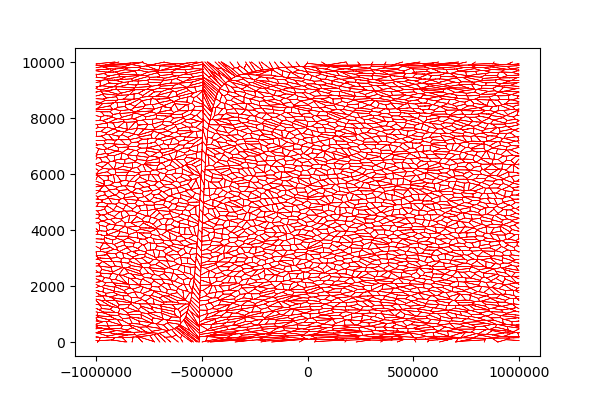
\includegraphics[width=0.7\linewidth]{evaluation/laguerre_tesselation_18}}}
	\caption{Plots of Laguerre Cells generated using a random mesh of $80 \times 40$ points initialised in geostrophic space using \ref{Initpoints} at (a) $6$ days (b) $9$ days $\Gamma = [-L,L]\times[0,H]$, where $L = 1\times10^6$ and $H = 1\times10^4$}
	\label{lagcells2}
\end{figure}
\newpage
\section{Total Energy as a Measurement of Error \label{energyerror}}
\begin{figure}[h]
	\centering
	\subfloat[]{{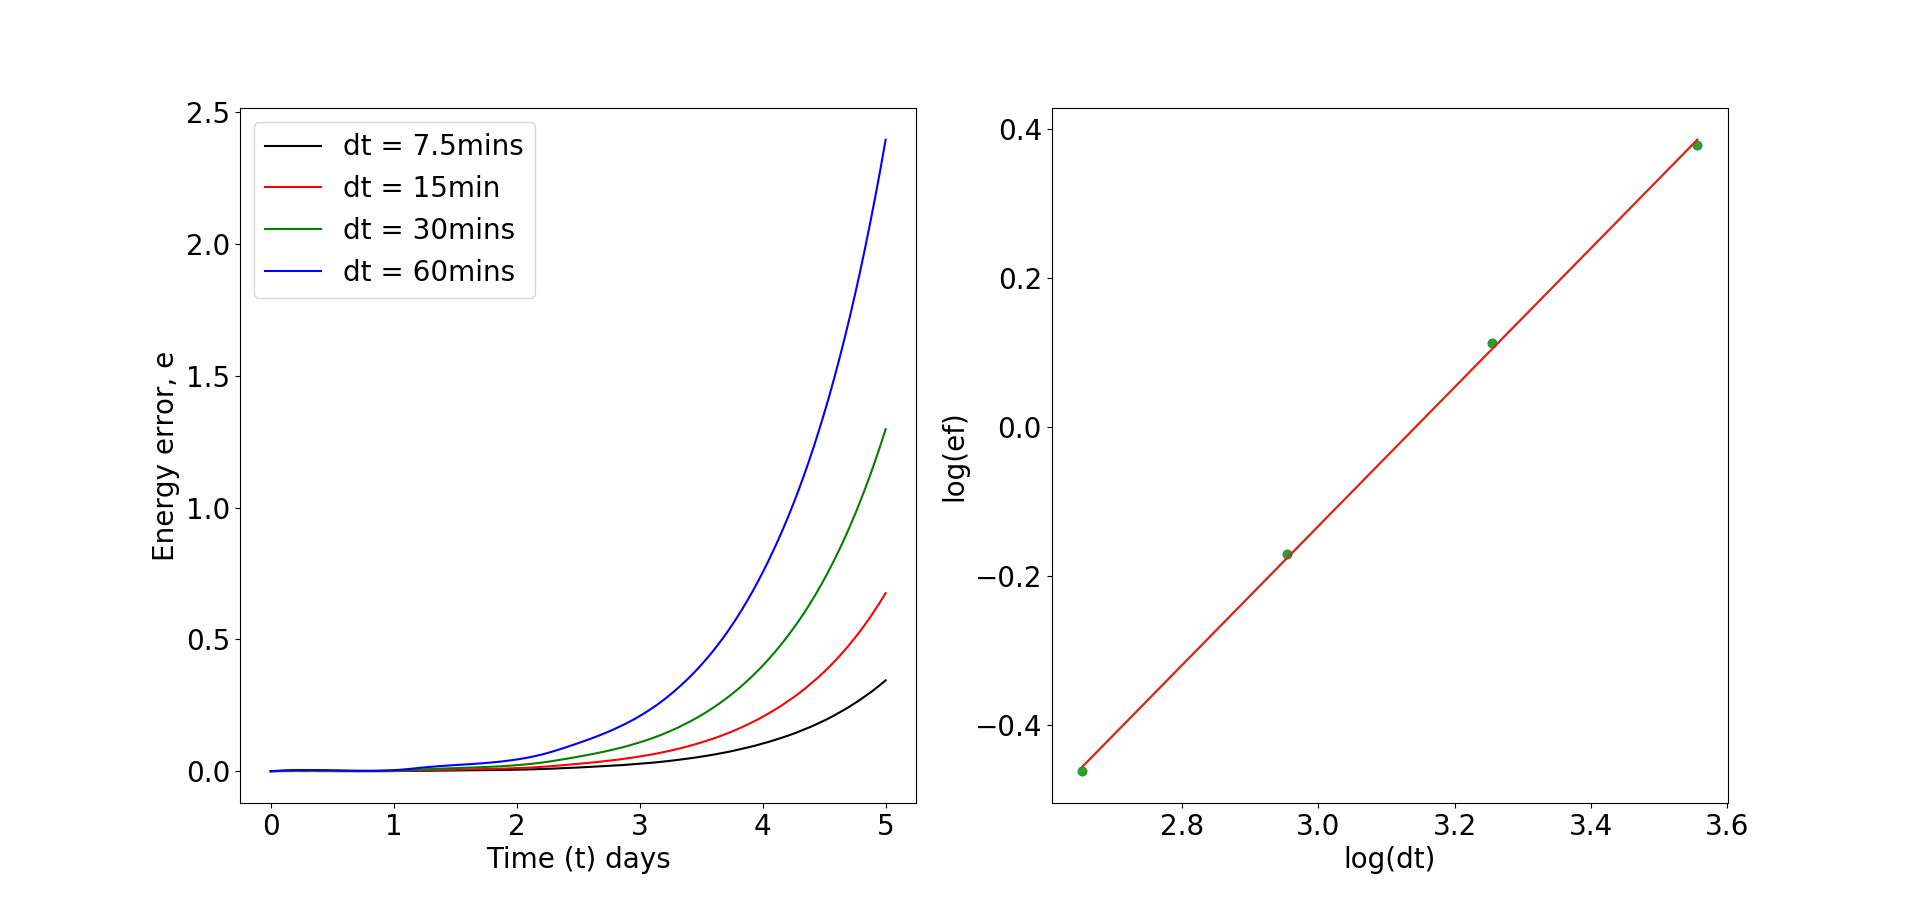
\includegraphics[width=0.9\linewidth]{evaluation/energy_5D_euler}}}\caption[Energy Error from implementation of SG/DA via Forward Euler timestepping method for 5 days]{Energy error following the implementation of SG/DA with a Forward Euler time stepping method for 5 days on a regular mesh of $80 \times 40$ points. $\log(\Delta t)$ vs. $\log(e_f)$. The line of best fit has gradient $m = 0.933$, 3.s.f} \label{fig:energy5deuler}
\end{figure}
\begin{figure}
	\subfloat[]{{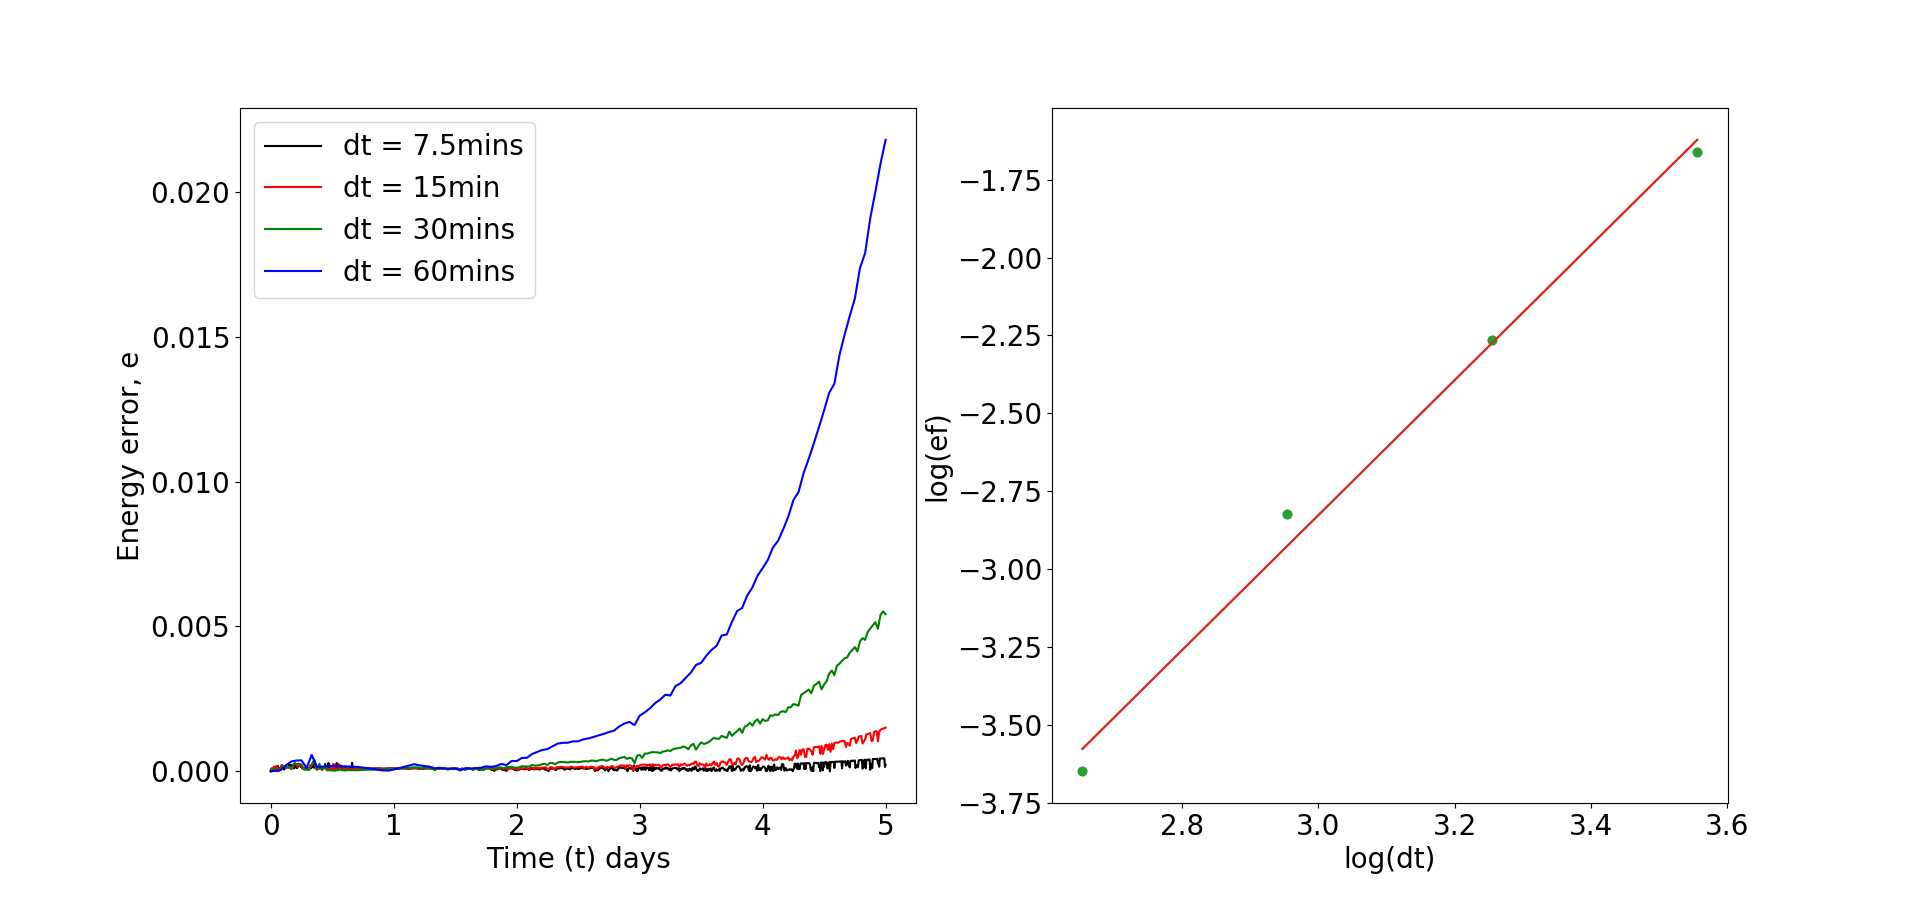
\includegraphics[width=0.9\linewidth]{evaluation/energy_5D_heun}}}\caption[Energy Error from implementation of SG/DA via Heun timestepping method for 5 days]{ Energy error following the implementation of SG/DA with a Heun time stepping method for 5 days on a regular mesh of $80 \times 40$ points. $\log(\Delta t)$ vs. $\log(e_f)$. The line of best fit has gradient $m = 2.17$, 3.s.f}
	\label{fig:energy5dheun}
\end{figure}
The aim of this section is to validate the results seen in section \ref{laguerre plots} above. With no known analytical solutions to the Eady model for frontogenesis \ref{EadyModel} that we are studying and with no numerical models achieving the resolution we are able to achieve with SG/DA a challenge arises in how to confirm that the results are suitable solutions for the Semi-geostrophic Eady model. In this case, we turn to the total energy to quantify the error in the implementation. This is justified as we know from \cite{Cullen2006a} that the total energy in equation \ref{EadyModel} is conserved. However, given the form of total energy from \ref{energy} as,

\begin{equation}
	E = f^2 \iint \frac{1}{2}\left(X-x\right)^2 - Z\left(z - H/2\right)\textrm{d}x\textrm{d}z
\end{equation}

There is a clear dependence on the values of the points in geostrophic space and the values of the centroids of their corresponding Laguerre cells. This indicates a dependence of the total energy of the system on the numerical solution given by SG/DA at each time-step. The graphs below show the total energy given by a system initialised from a grid of $80 \times 40$ points in geostrophic space (again from applying the transformation to points in physical space by \ref{Initpoints}). This time a regular mesh was used to ensure that the initial energy ($E_0$) was the same for each simulation. \\
\linebreak
The effect of decreasing the time step value was investigated for  both the Forward Euler and Heun time stepping schemes. In the following plots the energy error, $e_t$ is defined as $e_t = E_{t} - E_0$. The final energy error $e_f$ is used to create log-log plots confirming the relationship between the time step used and the numerical error of the implementation. What is most interesting in this is the gradient of the line of best fit, this gives an indication of the order of accuracy of the method. What we expect to see is a gradient, $m$, close to $m=1$ for the Euler method as this is well known to have a linear rate of converge \cite{Griffiths2010} and $m=2$ for the Heun method as this has a quadratic rate of convergence \cite{Griffiths2010}.
\newpage


\newpage

Figures \ref{fig:energy5deuler} and \ref{fig:energy5dheun} indicate promising initial findings. The straight lines in the log-log plots are clear evidence of a power law governing the error - time step relation. Moreover, the gradient values are reasonably close to what we were expecting.\\
\linebreak
The difference in computed values for the gradient to expected values is attributable to the error in applying the Damped Newton Algorithm in DA. To expand, rates of convergence are computed assuming $f(t,\bm{x})$ in $\frac{\textrm{d}\bm{x}}{\textrm{d}t} = f(t,\bm{x})$ has a Taylor expansion \cite{Griffiths2010}. In the case of SG/DA the right hand side includes the implementation of DA which carries error associated with the Damped Newton Algorithm. This is particularly visible in the Heun implementation where the error is significantly smaller. In this case the error associated with DA dominates that associated with the Heun's method and is seen as noise in the energy error curve.\\
\linebreak
Physically we can see that the energy error begins to grow the most between days $4$ and $5$, which coincides with the point where the front seen in figures \ref{fig: thetap ldiag1},\ref{fig: thetap ldiag2} begins to grow most rapidly. To investigate this further the energy error is found for a period of up to $10$ days.
\newpage
\begin{figure}[ht]
	\centering
	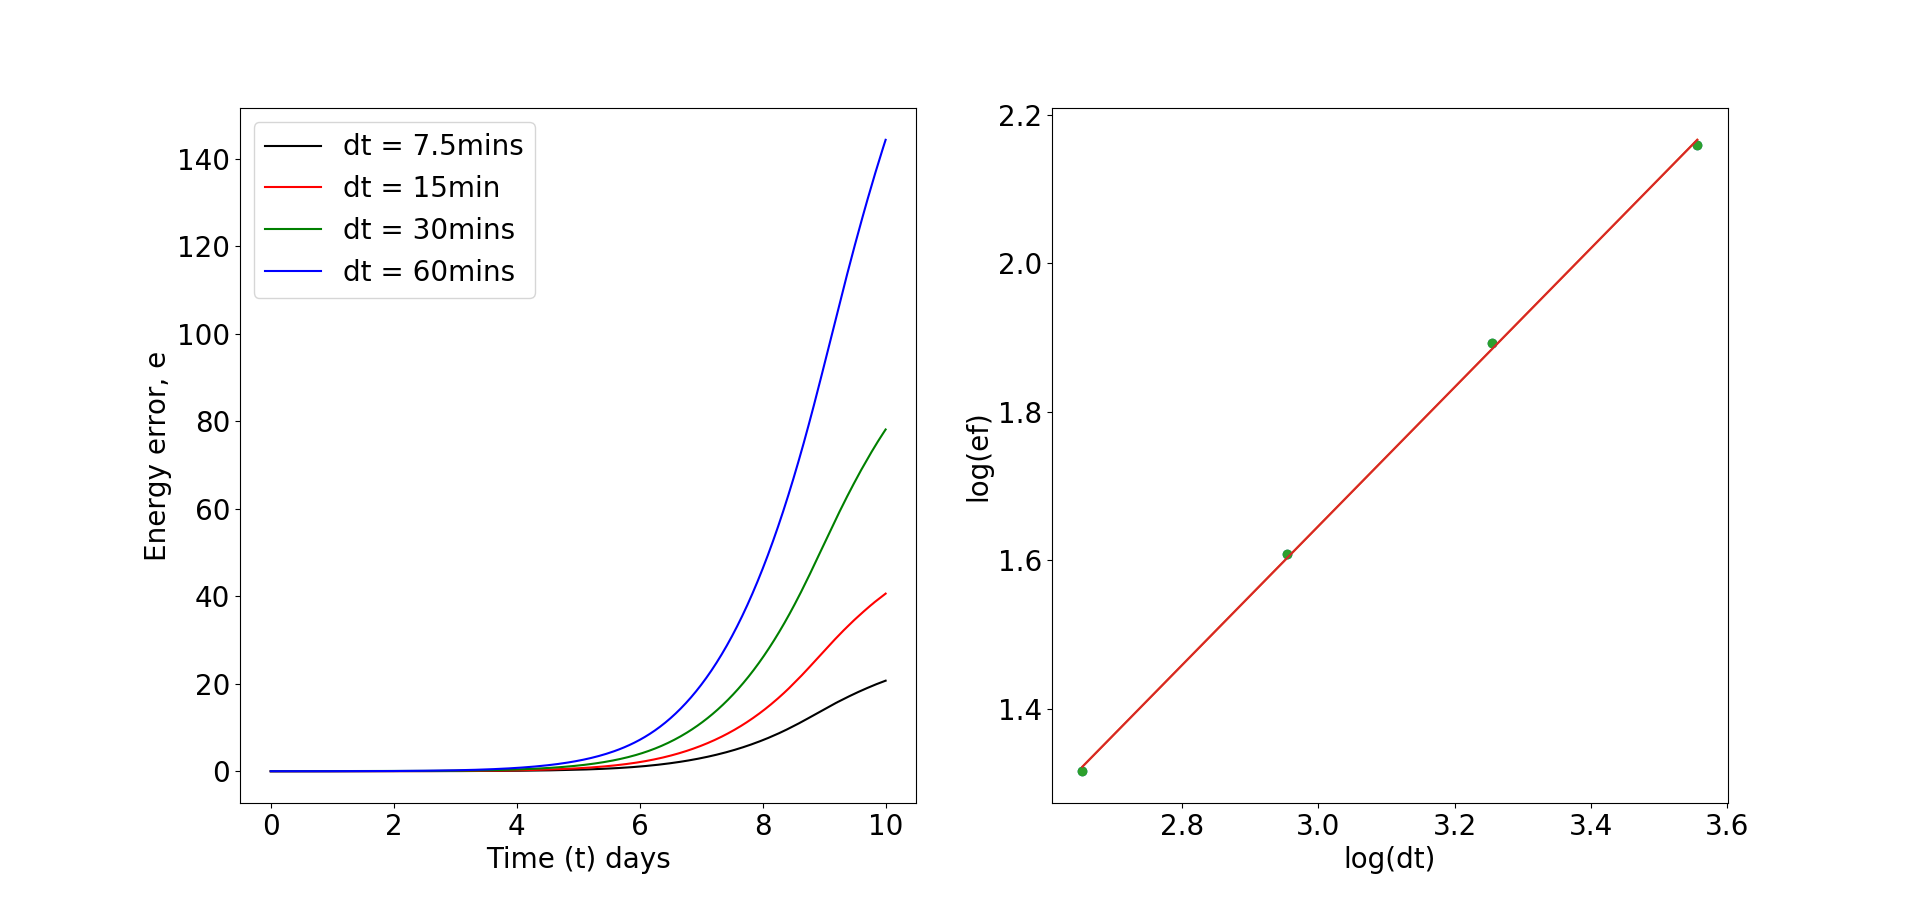
\includegraphics[width=1.1\linewidth]{evaluation/energy_10D_euler}
	\caption[Energy Error from implementation of SG/DA via Forward Euler timestepping method for 10 days]{(a) Energy error following the implementation of SG/DA with a Forward Euler time stepping method for 10 days on a regular mesh of $80 \times 40$ points.\\ (b) $\log(\Delta t)$ vs. $\log(e_f)$. The line of best fit has gradient $m = 0.935$, 3.s.f}
	\label{fig:energy10deuler}
\end{figure}
\begin{figure}[h]
	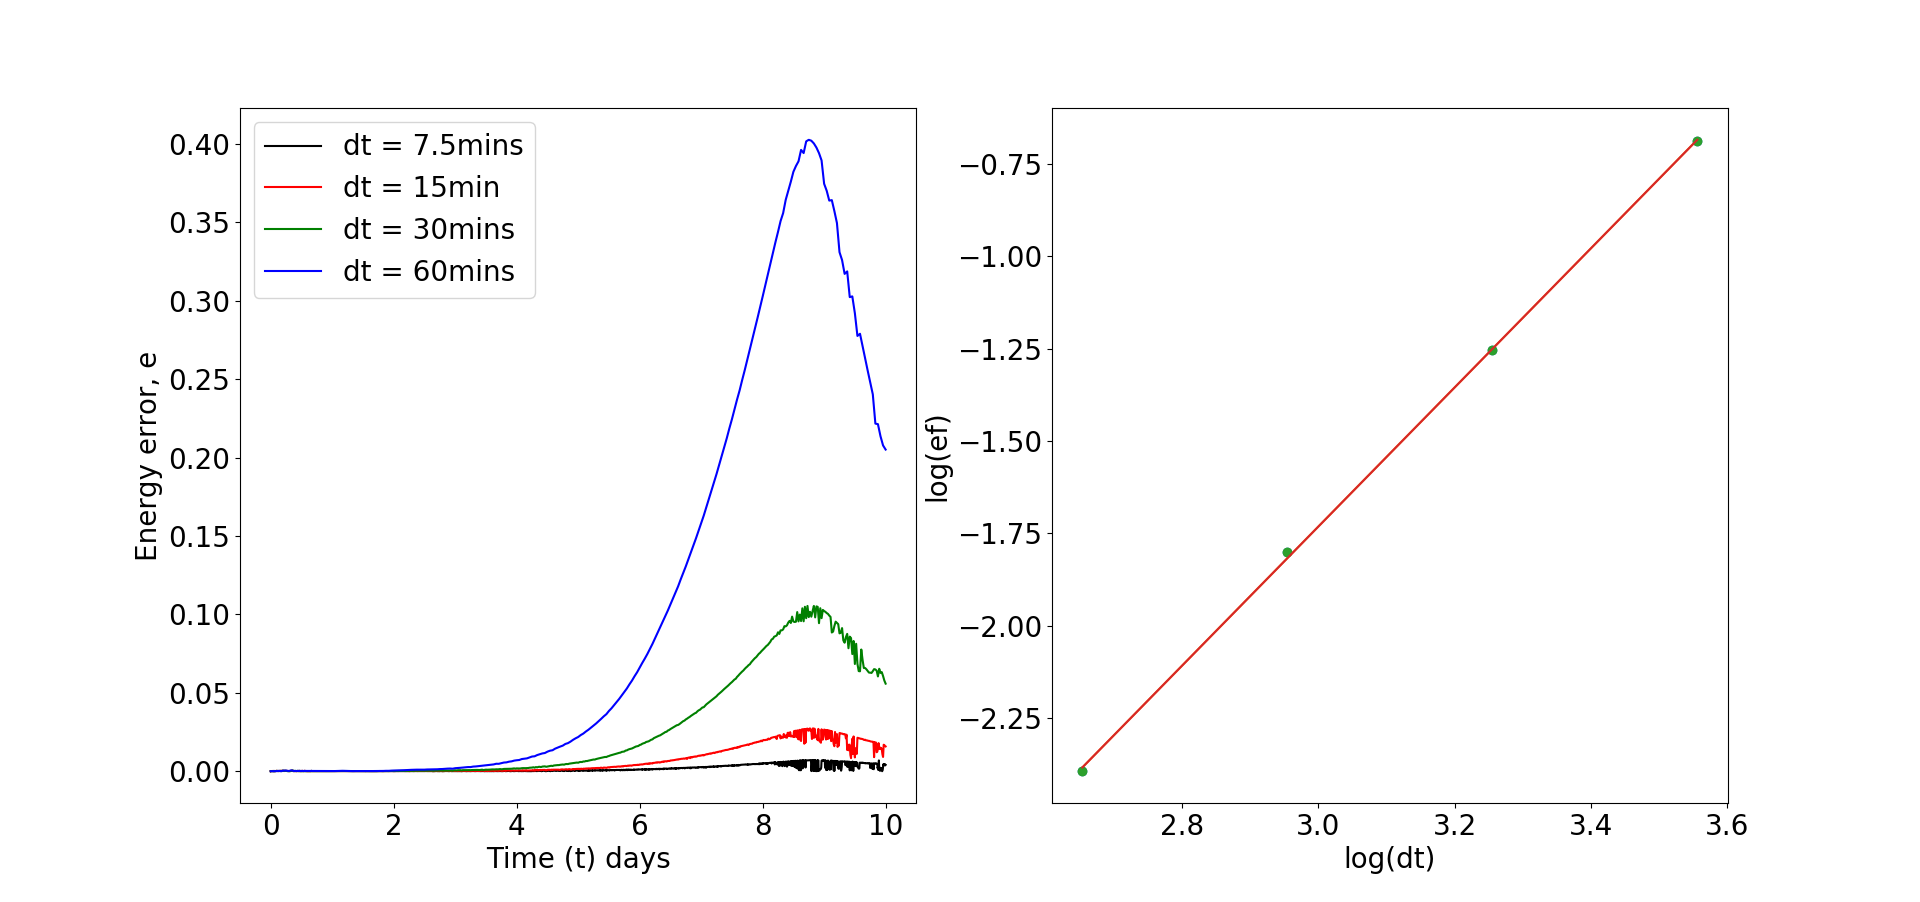
\includegraphics[width=1.1\linewidth]{evaluation/energy_10D_heun}
	\caption[Energy Error from implementation of SG/DA via Heun timestepping method for 10 days]{(a) Energy error following the implementation of SG/DA with a Heun time stepping method for 10 days on a regular mesh of $80 \times 40$ points.\\ 
		(b) $\log(\Delta t)$ vs. $\log(e_f)$. The line of best fit has gradient $m = 1.88$, 3.s.f}
	\label{fig:energy10dheun}
\end{figure}  
\pagebreak
\section{A Comparison of Time Stepping Methods \label{comparison}}

\begin{figure}[h]
	\centering
	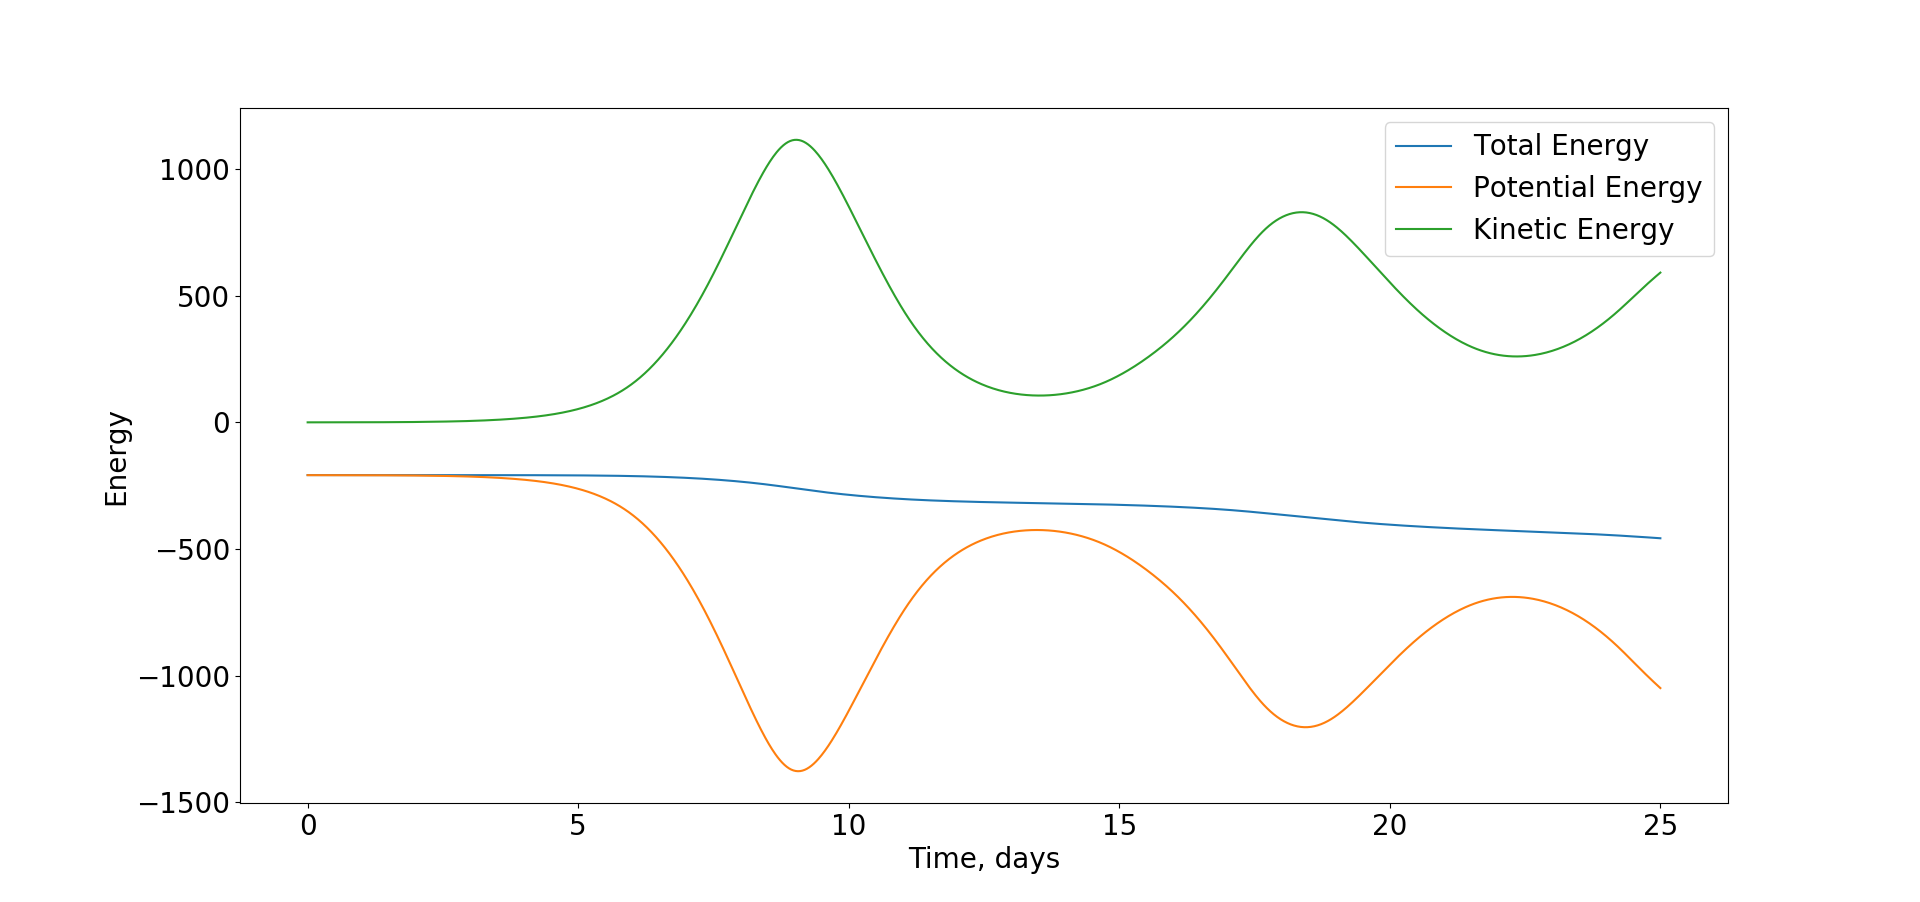
\includegraphics[width=0.8\linewidth]{evaluation/Energy_evolution_euler}
	\caption[Energy evolution for SG/DA with Euler time step scheme]{Energy evolution for SG/DA with Euler time step scheme for regular grid of initialised points}
	\label{fig:energyevolutioneuler}
\end{figure}

To validate the behaviour exhibited in section \ref{laguerre plots} we look at the behaviour of the Kinetic Energy, Potential Energy and Total Energy with time. We restate the energy in the form \ref{energy},

\begin{equation}
	E= f^2 \iint \frac{1}{2}\left(X-x\right)^2 - Z\left(z - H/2\right)\textrm{d}x\textrm{d}z
\end{equation}

The kinetic energy over the domain $\Gamma$ is defined by,

\begin{equation}
	E_{kin} = \int_\Gamma \ \frac{f^2}{2}(X-x)^2 \ dxdz
\label{KE}
\end{equation}

And the potential energy given by,

\begin{equation}
E_{pot} = \int_\Gamma \ - Z\left(z - H/2\right) \ dxdz
\label{PE}
\end{equation}

We now investigate the evolution of these quantities for a period of 25 days for each time stepping method, initialised with a regular mesh of $80 \times 40$ points transformed to geostrophic co-ordinates as in \ref{Initpoints}.
In figure \ref{fig:energyevolutioneuler} the cycle of frontogenesis and collapse is much clearer seen in the periodic nature of the Kinetic energy. The graph also shows that energy dissipation in the Forward Euler method is strongest after front formation.

\begin{figure}[h!]
	\centering
	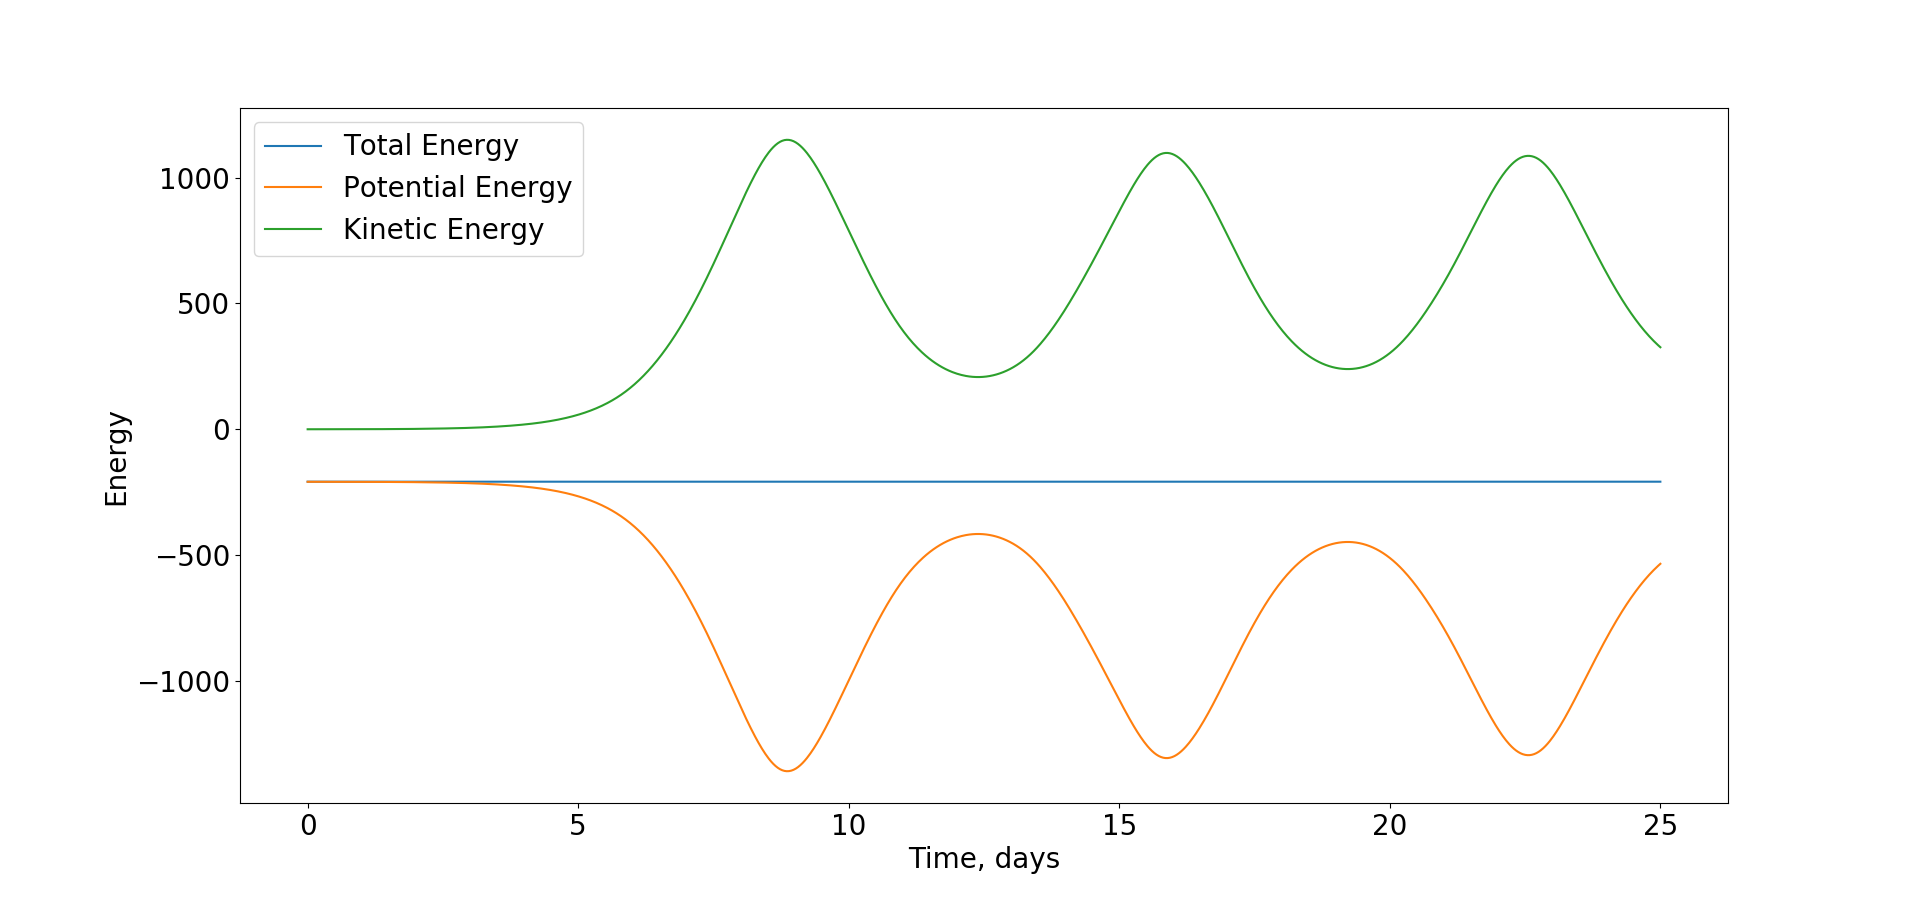
\includegraphics[width=0.8\linewidth]{evaluation/Energy_evolution_heun}
	\caption[Energy evolution for SG/DA with Heun time step scheme]{Energy evolution for SG/DA with Heun time step scheme for an initially regular grid of points}
	\label{fig:energyevolutionheun}
\end{figure}

From figure \ref{fig:energyevolutionheun} we see that Heun's method gives numerical results that appear to maintain energy conservation. Comparing the kinetic energy to that of the Forward Euler method there is significantly less damping in the cycle of front formation. The differences in behaviour of kinetic energy is explored further in \ref{fig:energyeulerheuncomparison}.
\\
\linebreak
The comparison in figure \ref{fig:energyeulerheuncomparison} shows a significant damping in the amplitude of oscillations in the Forward Euler time stepping scheme compared to the Heun scheme, where the second oscillation appears slightly damped but the third very similar in amplitude to the second. What is also striking is the difference in the periods of oscillation. The period of oscillation in Heun's method is significantly smaller and more uniform indicating a dispersion error in the Forward Euler implementation. 
\comments{\cite{Cullen2006a}period of oscillation}
\begin{figure}[h!]
	\centering
	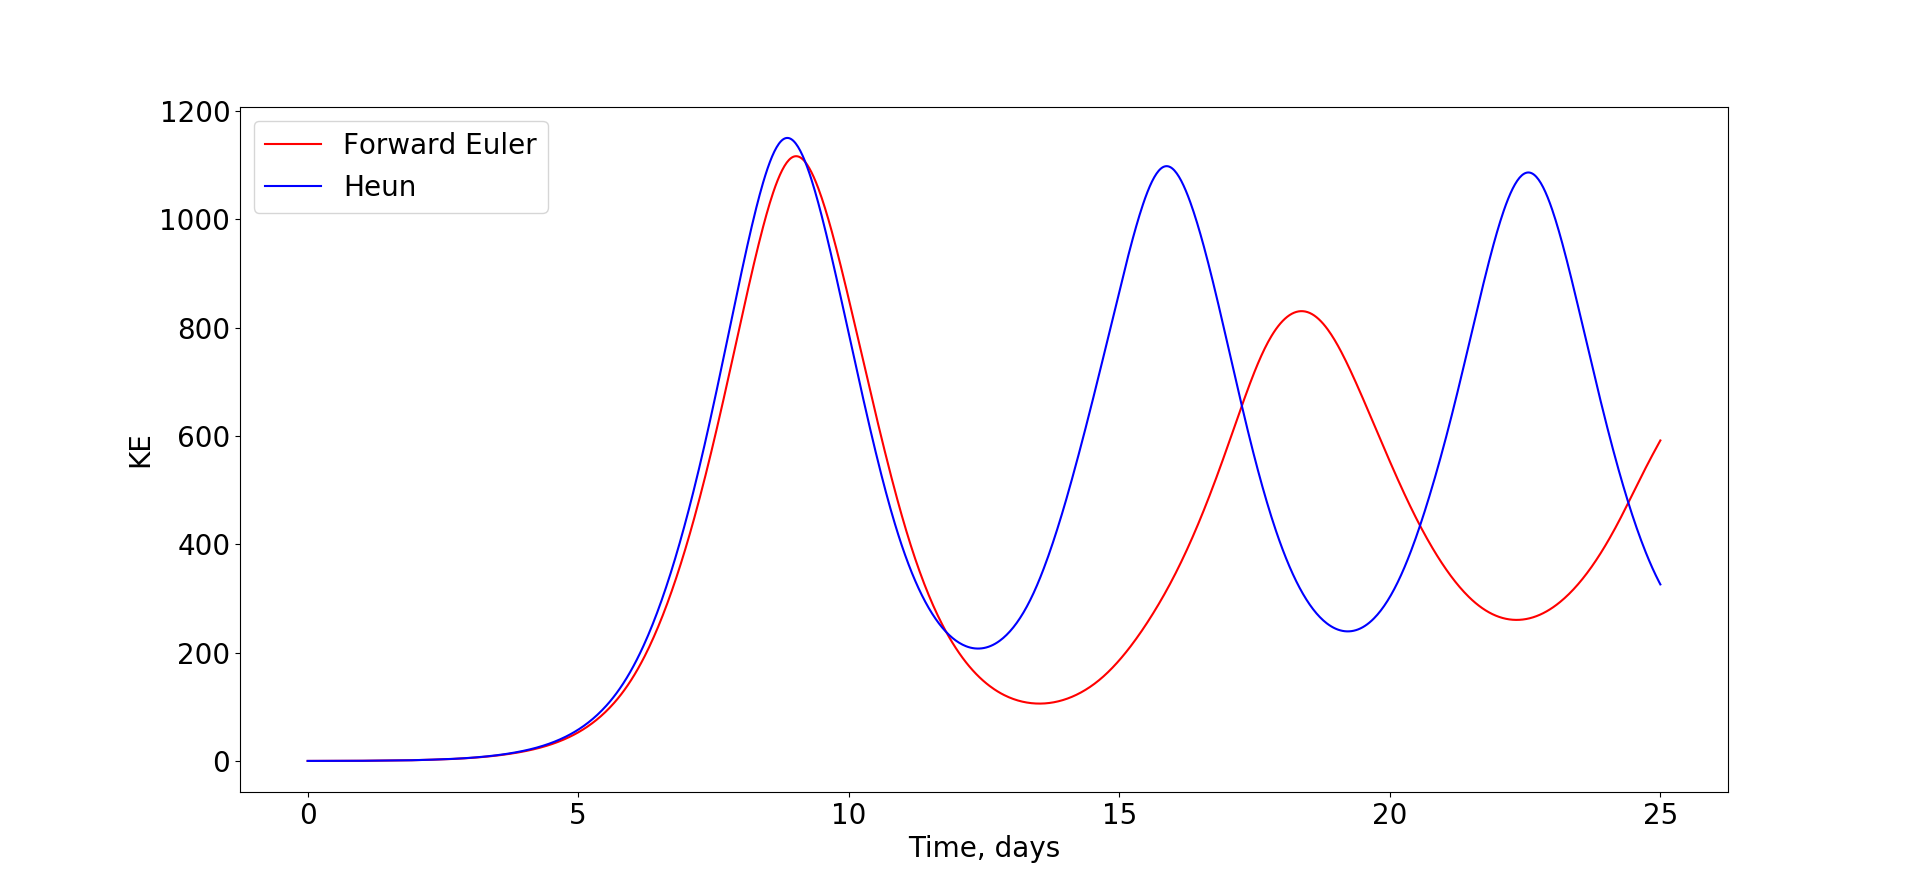
\includegraphics[width=0.9\linewidth]{evaluation/energy_euler_heun_comparison}
	\caption[Comparison of Energy Evolution for SG/DA with Heun/Forward Euler Time Stepping Schemes]{Comparison of energy evolution of solution of SG/EM with SG/DA for Heun and Forward Euler time-stepping schemes over a period of 25 days with a regular grid of initial points}
	\label{fig:energyeulerheuncomparison}
\end{figure}

\newpage
\section{Computational Performance}
The results of sections \ref{comparison} and \ref{energyerror} show a clear indication that using Heun's method for the time stepping of SG/DA gives a significantly more accurate result. However, considering that to implement Heun's method requires two calls to DA to solve the optimal transport problem at the prediction stage and correction stage the benefit of extra accuracy could be lost in a large increase to the runtime of the algorithm. Due to this we would expect the runtime of Heun's method to be close to twice that of Euler's method. In this section we investigate the additional time cost to running Heun's method in time stepping and evaluate whether this is justified.

\begin{table}[h!]
	\begin{tabular}{|c|c|c|} 
		\hline 
		$N$, ($2N^2$ points) & Runtime (s) FE Method & Runtime (s) Heun Method \\ 
		\hline 
		30 & 40.430 & 81.479 \\ 
		\hline 
		35 & 59.898 & 114.232 \\ 
		\hline 
		40 & 93.374 & 179.741 \\ 
		\hline 
		45 & 148.440 & 274.582 \\ 
		\hline 
		50 & 200.886 & 372.805 \\ 
		\hline 
		55 & 286.968 & 503.502 \\ 
		\hline 
		60 & 410.417 & 663.437 \\ 
		\hline
	\end{tabular}
\caption[Comparison of Runtime by Forward Euler and Heun's time step methods]{A comparison of runtime (seconds) by Forward Euler and Heun's time step methods using python cProfile package}
\label{table: runtime}
\end{table}

To compare the runtime of each time stepping method the python package cProfile was used around the time iteration part of the algorithm. Of course, this means that some set-up time costs are factored into the runtime measurement. From table \ref{table: runtime} it is already evident from table that the runtime of Heun's method is significantly greater than that of the Forward Euler method. Whilst for smaller values of $N$ the runtime is approximately doubles between implementing Euler and Heun's method we see that above $N = 45$ this relationship deteriorates.
\\
\linebreak 
To analyse this further we visualise the data from \ref{table: runtime} by plottin a best fit line for each method by linear regression using the \textquoteleft scipy.stats\textquoteright \ package available in python. 
\begin{figure}[h!]
	\centering
	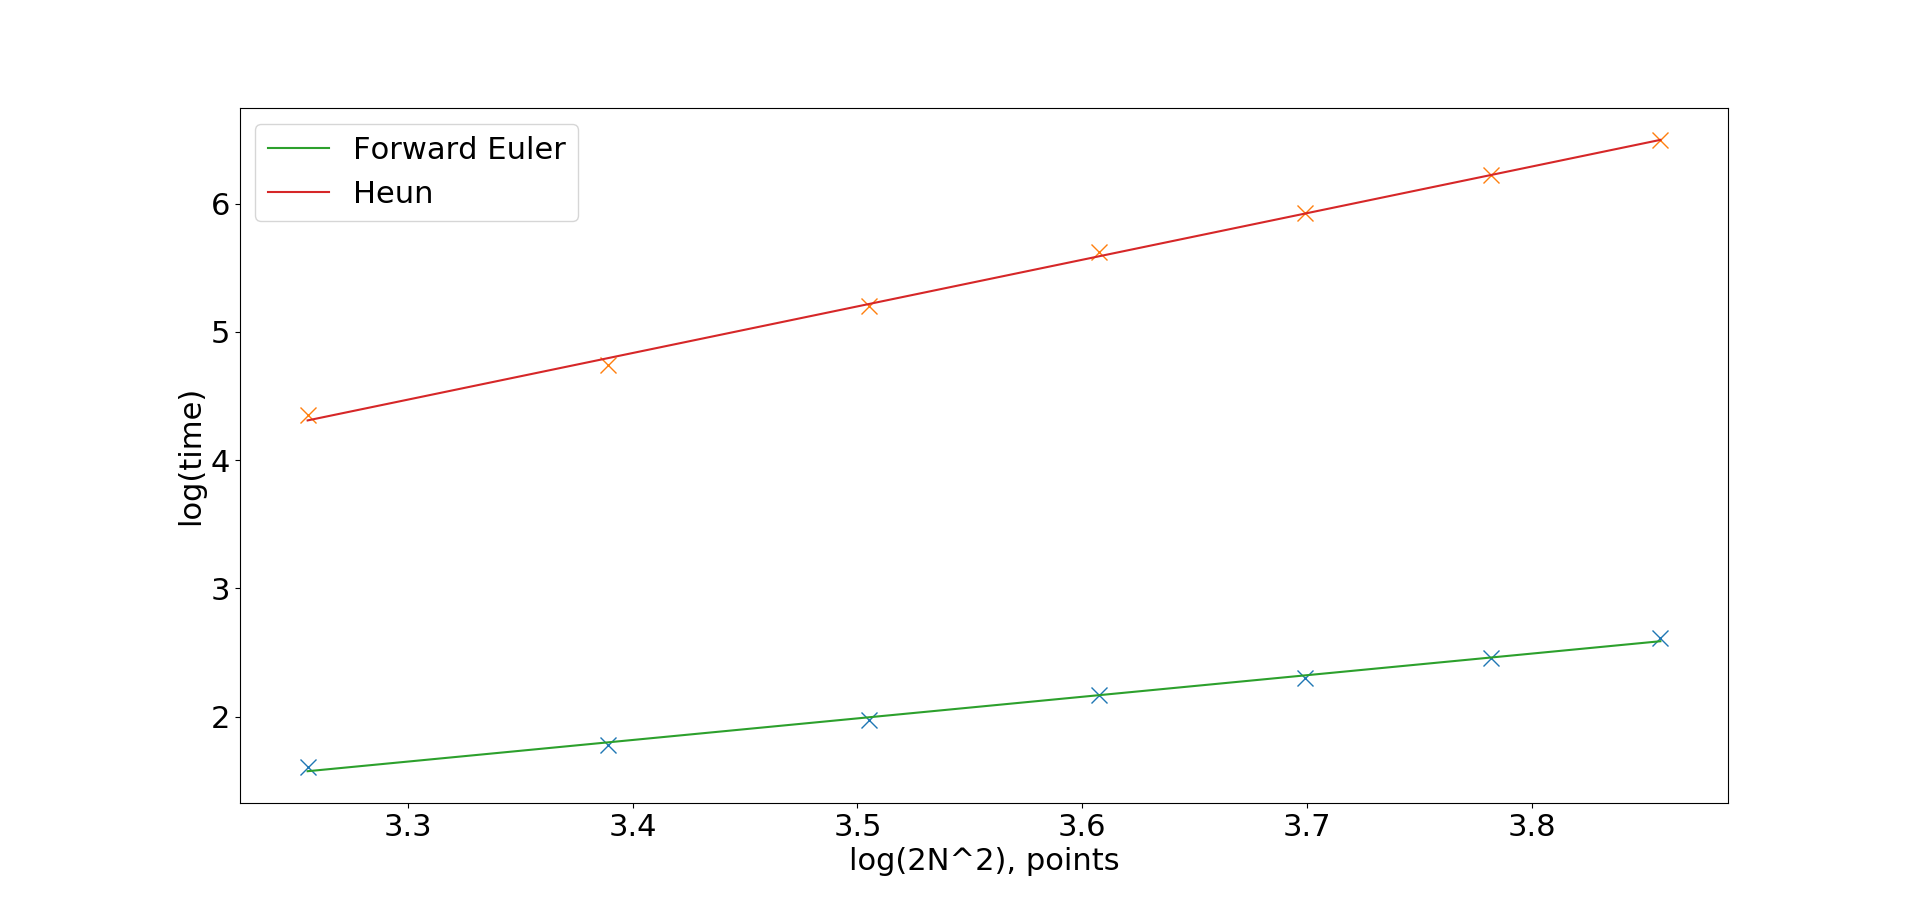
\includegraphics[width=0.95\linewidth]{evaluation/performance_loglog_plot}
	\caption[Time stepping performance based on number of points initialised in the domain]{Logarithmic plot showing $\log(2N^2)$ vs $\log(\textrm{runtime})$ for $N = (30,35,40,45,50,55,60)$ as in table \ref{table: runtime} and line of bestfit. The gradient of the line of bestfit for the Forward Euler method is $1.68$ 3.s.f and for $3.63$ 3.s.f for Heun's method using runtimes from \ref{table: runtime}}
	\label{fig:performanceloglogplot}
\end{figure}
\\
\linebreak
Figure \ref{fig:performanceloglogplot} highlights this disparity observed in the table we see that the gradient in the line of best fit of Heun's method is in fact $2.16$ times that of the Forward Euler method. Indicating another source of time cost in Heun's method. There are a number of reasons this could be. The additional time step calculation for the correction step of Heun's method would contribute to the increase in time cost. 
\\
\linebreak
From the cProfile results, which can be seen from running \textquoteleft SG\_DA\_performance.py \textquoteright \ (in the sg\_monge\_ampere repository) that the greatest time cost is in running DA to solve the optimal transport problem. This runtime could be reduced by recycling the weights from the previous time step as an initial guess for DA in the following time step. In practice this is harder to implement as the time stepping moves points in geostrophic space in the $Z$ direction. This means that the necessary condition for convergence, that the area of the cell associated with each geostrophic point is positive over the domain $\Gamma$ is not necessarily satisfied. Therefore the initial guess given by \ref{Initweights}  must be used for each call to DA. As the initial guess is most likely far from the final values of the weights this will greatly increase the time for DA to converge. As this is called twice in Heun's method this represents an additional cost to runtime which is not so easily quantified. A possible remedy for this is to perturb the values for the weights from the previous time step in such a way that the condition for initial positive cell area is satisfied. However, this is a non trivial problem.
\chapter{Conclusion}
\appendix
\chapter{First Appendix}

\bibliographystyle{unsrt}
\bibliography{bibs/MSc_Project}

\end{document}